% This file (dissertation-main.tex) is the main file for a dissertation.
\documentclass {udthesis}
% preamble

% Include graphicx package for the example image used
% Use LaTeX->PDF if including graphics such as .jpg, .png or .pdf.
% Use LaTeX->PS->PDF if including graphics such as .ps or .eps
% Best practice to not specify the file extension for included images,
% so when LaTeX is building it will look for the appropriate image type.
\usepackage{graphicx}
\usepackage[acronym]{glossaries}
\usepackage[inline]{enumitem}
\usepackage{amsmath}
\usepackage{caption}
\usepackage{subcaption}
\usepackage{url}
\usepackage{booktabs}
\usepackage{tikz}
\usetikzlibrary{matrix,shapes,arrows,positioning,chains}
\usepackage{threeparttable}
\usepackage{multirow}
\usepackage{tabularx}
\usepackage{multicol}
\usepackage[export]{adjustbox}

%%%%%%%%%%%%%%%%%%%%%%%%%%%%%%%%%%%%%%%%%%%%%%%%%%%%%%%%%%%%
% List of acronyms
%%%%%%%%%%%%%%%%%%%%%%%%%%%%%%%%%%%%%%%%%%%%%%%%%%%%%%%%%%%%

\newacronym{auv}{AUV}{Autonomous Underwater Vehicle}
\newacronym{rov}{ROV}{Remotely Operated Vehicle}
\newacronym{hov}{HOV}{Human Operated Vehicle}
\newacronym{api}{API}{Application Program Interface}
\newacronym{dyi}{DYI}{Do It Yourself}
\newacronym{ros}{ROS}{Robot Operating System}
\newacronym{dof}{DOF}{Degree of Freedom}
\newacronym{imu}{IMU}{Inertial Measurement Unit}
\newacronym{cad}{CAD}{Computer Aided Design}
\newacronym{lipo}{LiPo}{Lithium Polymer}
\newacronym{tcp}{TCP}{Transmission Control Protocol}
\newacronym{acp}{AC}{Alternating Current}
\newacronym{dcp}{DC}{DIrect Current}
\newacronym{fps}{FPS}{Frames Per Second}
\newacronym{ar}{AR}{Augmented Reality}
\newacronym{rst}{RST}{Rotation, Scaling and Translation}
\newacronym{fov}{FOV}{Field of View}



\makeglossaries
\graphicspath{{fig/}}

\begin{document}

%=========================================================================================
% Scallop recognition

\chapter{Distance based Global Descriptors for Multi-view Object Recognition}
\label{chap:dist_des}

%================================================================================================================
\section{Introduction}
\begin{enumerate}
	\item The ability to recognize objects enables a robotic system to interpret its environment and make intelligent decisions based on the identity of the objects around it.
	
	\item To recognize objects from images, prior information about appearance of the object is required.
	
	\item The appearance of the object is encoded in form of features which an object recognition system can extract and through it decode the identity of the object by the application of machine learning methods.

	\item To unambiguously distinguish between multiple objects, the information encoded in the object features extracted from a single image needs to be sufficiently discriminative.
	
	\item In cases where information available in a single image of a target object is insufficient to determine its identity, multiple-views of the target can be combined to gather information sufficient to unambiguously identify an object.
	
	\item The idea of combining multiple sensor measurements comes under the purview of active sensing.

	\item In the computer vision domain, using multiple views of an object methods are closely related to class of multi-resolution or image pyramid based techniques.

	\item Since the task of separating the background from foreground pixels in an image becomes problematic in the absence of sharp edges and in the presence of noise, object recognition techniques that can extract information from an image offer a way to detect the presence of a target object in an image.
		
	\item In this paper, we propose an object recognition method that combines information from multiple views of a target acquired from a series of heights, to build a feature descriptor that can operate on an image without segmentation of foreground and detect the presence of a target object.	
\end{enumerate}

Object recognition from noisy images is critical for robotic systems that operate on natural environments that are prone to noise in measurements. In the presense of noise, the information contained in an image featuring an \emph{object-of-interest} might not be sufficient to unambiguously make a decision on the identity of an object. The idea of combining information from multiple views of an offers an avenue to resolve this ambiguity in the object's identity. This object recognition method proposed here is a machine learning framework that combines information from multiple views of a target and employs global image descriptors to solve a binary classification problem.

Object recognition can be cast as a generalized machine learning problem. Traditional machine learning approaches \cite{alpaydin} use a learning set with annotated instances to learn the characteristics of an object. If the pixels of an object are presegmented in a test image, machine learning classifier can be used to label the given instance as a target object if sufficient proof is available from the learning set to support this hypothesis. Machine learning techniques like convolution neural networks \cite{cnn} use several thousand of labeled image instances to solve the object recognition problem in a purely data-driven fashion. In the absense of large datasets for specialized applications like underwater animal recognition, such data-driven approaches require a labor intensive annotation process.

An alternative to data-driven approach is a feature based object recognition approach \cite{roth} where prior knowledge about the object to be recognized can be leverage to build specialized feature descriptors that capture the appearance traits of an object. The models used in such cases can range from simple geometric shapes to complex free-form models \cite{campbell, belongie}. The feature descriptors thus trained encode the object appearance through a low-dimensional mathematical model. This model can be used to check for the presence of an object in an image.

Feature based approaches can be further subdivided into two classes; local and global feature based approaches. Local feature based approaches like \gls{sift} \cite{sift} and \gls{surf} \cite{surf} encode a configuration of localized features specific to an object to build a descriptor for an object. In the case of \gls{sift} and \gls{surf}, feature descriptors obtained are also invariant to in-plane rotation and scaling making them very robust for a multitude of object recognition appraches. However, since local descriptors primarily depend on artifacts like corners in images, they can be severely affected in the presence of noise which can degrade sharp edges and corners in an image. On the otherhand, global feature descriptors like gist \cite{gist} are more resilient to noise as they encode general characteristics of an image which is less impacted by the presence of noise. Global feature representation also have the additional benefit of not requiring segmentation which in itself is a hard problen to solve in noisy images where it is difficult to delineate foreground and background regions. However, the global feature descriptors often only provide a weak description of an object which might not be sufficient to unambiguously detect the presence of a specific object

One approach to strengthen a weak feature descriptor is to combine information from multiple information sources derived from a single object instance. A way to accomplish this is by merging information from multiple views of an object. Such an approach is more reliable than a case where a single view of an object does not contain sufficient information to suggest the presence of an object. A hypothesis test on each of the multiple views can then be combined to eventually classify the object. This process of combining multiple weak classifiers is a common theme in machine learning constructs like boosting and bagging \cite{alpaydin}.

The idea of combining multiple sensor measurements is seen in the field of active sensing \cite{chen}. In most active sensing problems, like \emph{next best view} \cite{roy,dunn}, the task is to find subsequent sensor positions to collect data that is intended to increase the knowledge associated with a target object. Using multiple views a target from predetermined sensor positions similar to active sensing in terms of combining information from multiple view of an object to learn more about the but nevertheless offers differences in the way the final objective of object classification is accomplished.

Combining information from multiple height can also be related to computer vision techniques that operate on the principle of multi-resolution processing or image-pyramid based method. Visual attention based object recognition framework VOCUS \cite{frintrop} and multi-resolution pedestran detection \cite{park} utilizes features from multiple scales to build a robust feature descriptor for objects. These multiresolution techniques essentially resize an image to compute features at different scales. Thus such techniques can only represent the information available from a single parent image in different forms. In cases where objects exhibit different appearance traits when viewed from different heights, multiple images of an object are needed to capture new information disclosed at different scales.

In this chapter, we propose an object recognition technique that combines information from multiple images of an object gathered from different heights to perform binary classification. The contribution here is in design of a novel histogram-based global feature descriptor along with a hypothesis testing mechanism that combines information from multiple-views of a target object. The approach developed here lies at the intersection global feature descriptors, active sensing and multi-resolution image processing to offer a novel way abject recognition technique that is intended to operate on noisy natural images. The use of global feature descriptors avoids the difficult task of segmentation in noisy images and at the same time enables to construct a strong feature descriptor by combining information from several weak descriptors learnt from each height scale.

%================================================================================================================
\section{Preliminaries}

\subsection{Grabcut-in-one-cut Algorithm}
\label{sec:onecut}

\begin{enumerate}
	\item When initialized with foreground and background seed pixels, graphcut treats the segmentation problem as a binary graph partition problem to separate the foreground pixels from background.
	
	\item To perform the binary partition of foreground and background, graphcut checks for similarity or dissimilarity of the pixels neighboring the input foreground and background seeds till a complete binary partition is achieved through labeling of all points in an image as either foreground or background.
	
	\item If the location of an object in an image is known, graphcut segmentation offers a method to segment the image into foreground and background pixels.
\end{enumerate}

Graphcut algorithm treats the segmentation problem as a graph partition problem \cite{mincut_maxflow}. Consider a case where each pixel $p \in \mathcal{P}$ of an image is treated as a vertex $i$ in the graph $G(\mathcal{V},\mathcal{N})$. Two neighboring pixels $p$ and $q$ represented by vertices $i$ and $j$ respectively are connected by an edge $e_{ij}$ in the graph $G$. The task of binary partition of this graph $G$ into foreground and background pixels is cast into an optimization problem where the energy $E$ is to be minimized. The energy $E$ here is formulated as 
%
\begin{equation}	\label{eq:graph_partition}
  E(L)=\sum\limits_{p_i\in \mathcal{P}} D_p(L_p)+\sum\limits_{(p,q)\in \mathcal{N}} V_{p,q} (L_p,L_q),
\end{equation}
%
where $L_p$ corresponds to a labeling of pixel $p$, $D$ is a data penalty function that assigns a likelihood for pixel $p$ to belong to either foreground or background label class, $V_{p,q}$ is an interaction potential function that encourages spatial coherence by penalizing discontinuity in label values of pixels. A binary partition of this graph is obtained by choosing a label for each pixel $p$ such that the energy $E$ of the image is minimized. This graph-based segmentation theory, also referred to as max-cut min-flow algorithm was was adapted in \cite{onecut} to suit the binary image segmentation problem. To this end, a variant of graphcut, the Grabcut-in-one-cut \cite{onecut} uses pre-specified foreground and background seeds to perform a binary partition of an image. According to Grabcut-in-one-cut algorithm \cite{onecut}, the energy function in \eqref{eq:graph_partition} is reformed as
%
\begin{equation} \label{eq:graph_partition_onecut}
  E_{seeds}(S)=-\beta \| \theta^S-\theta^{\bar{S}} \|_{L_1}+\lambda|\partial S|\,.
\end{equation}
%
Here $\theta^S$ and $\theta^{\bar{S}}$ are the histograms of the foreground and background pixels in the image. The first term of \eqref{eq:graph_partition_onecut} penalizes the pixels with intensities that overlap with both the foreground and background distributions. The second term $|\partial S|$ of \eqref{eq:graph_partition_onecut} is a term analogous to $V$ in \eqref{eq:graph_partition}, that tries to enforce similar labeling of neighboring pixels and therefore penalizes a change in labeling across neighbors. The weights $\lambda$ and $\beta$ allow to vary the contribution of the first and second term to the value of the energy function in \eqref{eq:graph_partition_onecut}. Finally the $L_2$ in \eqref{eq:graph_partition_onecut} refers to the $L2$-norm.

The algorithm proposed in \cite{onecut} generates a binary partition of an image into background and foreground by extrapolating the input foreground and background seed pixels. If there is an automated means to find the location of foreground objects, the seeds required by this algorithm can be automatically generated hence making this guided segmentation approach fully autonomous.

\subsection{Data Collection Apparatus}

%======================================================================================================
\subsubsection{Imaging Rig}
\label{sec:imaging_rig}

\begin{enumerate}
	\item The imaging rig comprises a frame with a camera holder that allows the camera to be positioned at different heights from the ground.
\end{enumerate}


The imaging rig shown in Figure~\ref{fig:im_rig} allows a camera to be held at different heights from the ground for imaging experiments. The height bar slides up or down and can be locked at a specific configuration through specially designed holders on the scaffold support of the imaging rig. By varying the position of the height bar, the height of the camera holder that is attached to the lower end of the height bar can be varied. This allows the camera held on to the camera holder to capture images of targets placed on the ground from different controlled heights. The camera holder was designed to hold a GoPro Hero 4 camera \cite{gopro}.
	
\begin{figure*}
  \centering
  \begin{subfigure}[]{0.45\textwidth}
      \includegraphics[width=\textwidth]{imaging_rig_labeled}
      \caption{}
      \label{fig:im_rig_side}
  \end{subfigure}
  \begin{subfigure}[]{0.45\textwidth}
      \includegraphics[width=\textwidth]{imaging_rig_top_scaled}
      \caption{}
      \label{fig:im_rig_top}
  \end{subfigure}
\caption[Imaging rig used for data collection in multi-image object recognition approach]{The imaging rig allows the height bar to slide up or down, thereby letting the height of the camera from the ground to be varied. The different components of the imaging rig are labeled in Figure~\ref{fig:im_rig_side}. The camera holder attached to the lower end of the height bar is designed to carry a GoPro Hero 4 camera.}
\label{fig:im_rig}
\end{figure*}	

%======================================================================================================
\subsubsection{Imaging Environment}


\begin{enumerate}
	\item Since underwater object recognition could pose a challenging problem due to presence of noise and lighting variations, data was collected in a test tank filled with water.
\end{enumerate}


Environment where object recognition experiments are performed could affect the performance of an algorithm. In case of an environment with limited to no control over the imaging parameters, the level of noise introduced into the sensor measurements is difficult to gauge for taking any corrective recourse. To avoid such difficulties, it might be tempting to perform object recognition experiments in controlled laboratory conditions, thereby allowing the possibility to tune the environmental parameters to enhance the performance of an algorithm. However if an algorithm is intended to operate on natural images, there are often going to be unpredicatble variations in environmental factors that could adversely affect the performance of an algorithm. In such a case, to accurately validate an algorithm that is intended to operate on natural environments, it is imperative to choose a 
test environment where the conditions are close to the expected natural conditions. Following this line of reasoning, since this object recognition algorithm is intended to operate on noisy natural environments, an underwater environment with uncontrolled lighting was chosen as the test environment. A circular tank in the Robot Discovery Lab (RDL) at University of Delaware filled with 4 feet of fresh water was thus utilized to collect experimental data. The imaging rig described in Section~\ref{sec:imaging_rig} was submerged inside this test tank during the data collection process.

%======================================================================================================
\subsubsection{Object Specimens}


\begin{enumerate}
	\item To validate the developed multi-image recognition method, commonly available produce like orange and strawberry were selected as they offered specimens with natural intra-class along with significant inter-class differences in appearance.
\end{enumerate}


The focus of this work is to recognize a class of objects that can exhibit some level of intra-class variance that is characteristic to naturally occurring objects. One such example is underwater marine organisms, where each species can have several identifiers that distinguish them from a different species. However in most cases, the members of a single species also exhibit some level of variation in their appearance. To accommodate such cases, the specimens used to validate this multi-image algorithm were required to have \begin{enumerate*}[label=(a)]  \item some characteristics that are unique to the class they belong to \item small variations with regards to appearance within the same class of objects \item easy accessibility for experimentation purposes. \end{enumerate*} All these points were satisfied by natural produce like potatoes, oranges, tomatillos and strawberries. Natural produce exhibit significant inter-class variance, sufficient intra-class variance and are readily available in stores making 
them ideal 
candidates for object specimens. Figure~\ref{fig:produce_species} shows an assortment of potatoes and tomatillos to visually reinforce the inter-class and intra-class variance exhibited by naturally occurring objects. The underwater data on which this multi-image algorithm is validated is composed of a set of 10 oranges and 13 strawberries.
%
\begin{figure*}
  \centering
  \begin{subfigure}[]{0.45\textwidth}
      \includegraphics[width=\textwidth]{potatoes_species}
      \caption{Potatoes}
      \label{fig:potato_species}
  \end{subfigure}
  \begin{subfigure}[]{0.45\textwidth}
      \includegraphics[width=\textwidth]{tomatillos_species}
      \caption{Tomatillos}
      \label{fig:tomatillo_species}
  \end{subfigure}
\caption[Illustration of the inter-class and intra-class variance exhibited by naturally occurring objects]
{An illustration of the inter-class and intra-class variance exhibited by naturally occurring objects like 
potatoes (Figure~\subref{fig:potato_species}) and tomatillos (Figure~\subref{fig:tomatillo_species})}.
\label{fig:produce_species}
\end{figure*}	
%
%================================================================================================================
\section{Definitions}

\subsection{Histogram Signature}
\label{sec:hist_signature}

As a part of this object recognition technique we define a histogram signature that is an improvement on the generic histogram, specifically designed to deal with possible noise in the pixel values. The rest of this section defines this histogram signature.

The generic histogram $H_f:b_i\to n_i$ of some colorspace $f$, with $n_i$ representing the count of bin $b_i \in \mathcal{B}$, captures the distribution of values of pixels in colorspace $f$ in an image. Any pixels affected by noise in image $I$ could corrupt the histogram $H_f$. If we assume that $e\%$ of the pixel values of an image constitutes noise, then the histogram $H_f$ can be reformulated to reject the bins containing $e\%$ of pixel values that are least likely to occur as dictated by the histogram $H_f$ itself. Before computing the refined version of this histogram, the histogram $H_f$ is first normalized to get $\bar{H}_f:b_i\to \bar{n}_i$ as shown in \eqref{eqn:hist_norm}.
%
\begin{align}	\label{eqn:hist_norm}
 \bar{H}_f(b_i)=\frac{n_i}{\sum_{j}n_j}=\bar{n}_i
\end{align}
Now the refined histogram signature $\mathcal{H}_f:b_i\to n'_i$ is computed, such that
\begin{align}
  n'_i = 
  \begin{cases}
     \bar{n}_i & b_i \in \mathcal{B}_e\\
     0	&	b_i \in \bar{\mathcal{B}}_e
  \end{cases},
\end{align}
%
where $\mathcal{B}_e$ and $\bar{\mathcal{B}}_e$ constitute a binary partition of $\mathcal{B}$, 
i.e. $\mathcal{B}_e \cap \bar{\mathcal{B}}_e = \phi \text{ and } 
\mathcal{B}_e \cup \bar{\mathcal{B}}_e = \mathcal{B}$. 
The set $\bar{\mathcal{B}}_e$ is chosen such that 
$\bar{\mathcal{B}}_e$ is the smallest cardinality subset of 
$\mathcal{B}$ that satisfies the condition $\sum_{b_i \in \bar{\mathcal{B}}_e} \bar{H}_f(b_i) > 1-e$. 
The formulation of set $\bar{\mathcal{B}}_e\subseteq\mathcal{B}$ can be restated as
\begin{align}
 \mathcal{{B}}_e=\underset{|\bar{\mathcal{B}_e}|} {\mathrm{argmin}} \sum_{b_i \in \bar{\mathcal{B}_e}} \bar{H}_f(b_i) > 1-e
\end{align}

Ultimately the $|\mathcal{B}|$-element histogram signature $\mathcal{H}_f$ encodes the histogram information while attempting to prevent noise present in sensor measurements from corrupting the computed histograms of an image.

\section{Methodology}
\label{sec:distdes_methodology}

\begin{enumerate}
	\item Any machine learning technique like the one used here for object recognition comprises a learning and a testing phase.
	
	\item The learning phase of object recognition involves extracting features that are capable of identifying a target unambiguously.
	
	\item The testing phase is the application of the learned machine learning model to an application where the identity of an object is to be ascertained.
	
	\item To validate the developed theory, an image dataset with images of objects captured from different known heights was gathered.
\end{enumerate}	


The algorithm developed in this paper is a form of machine learning technique. As in other machine learning techniques, there are two parts: learning and validation. In the learning phase features and other attributes of an object class are captured from labeled instances of the object available in the learning set. In the validation phase, the learned descriptor for an object class is validated against pre-labeled images to evaluate the performance of an algorithm. The data collection and annotation phases that provides data used for learning and testing parts of this algorithm is also discussed in detail.

\subsection{Data Collection}
\label{sec:distdes_data_collection}

\begin{enumerate}
  \item 13 Images of each target is captured between heights of 32in and 8in with an interval of 2in.
\end{enumerate}	


The data collection involves capturing 13 images of each object specimen. For the validation of this multi-image object recognition algorithm, data was gathered from 23 specimens (10 oranges and 13 strawberries) bringing the total images collected to $299\, (23 \times 13)$. Each specimen was first placed on the floor below the camera-holder on the imaging rig (see Figure~\ref{fig:im_rig}). The height bar was moved up till the camera holder was $32$ inches away from the ground. A GoPro Hero 4 camera attached to the holder was then triggered to capture an image of the specimen. This image captured the visual appearance of the specimen 32 inches away from the ground. Following capturing the first image, without disturbing the object, the next image was captured after lowering the height bar such that the camera is now $30$ inches away from the ground. Another image of the specimen is now captured. 
This process of lowering the camera by 2 inches between subsequent images is continued till the camera gets to a height of $8$ inches away from the ground. 
The series of images captured from a height of 32 inches to 8 inches with an interval of 2 inches between images results in 13 images per specimen. 
These 13 images capture the appearance of a specimen from different heights. An illustration of the 13 images captured per specimen for an instance of strawberry and orange is shown in Figure~\ref{fig:height_specimen}. An important point to note here is the imaging rig is handled manually between each image capture which sometimes leads to displacement of the imaging rig or the specimen on the ground. 
Additionally disturbances in the underwater environment where the specimen was placed added another source of inconsistency that sometimes lead to the specimen or the imaging rig getting displaced during the data collection process. 
Since natural environments are uncontrolled, these uncontrolled factors in the data collection process add some level of beneficial variation to the gathered dataset which in turn could make the machine learning algorithm robust to such variations.

\begin{figure*}
  \centering
  \begin{subfigure}[]{\textwidth}
      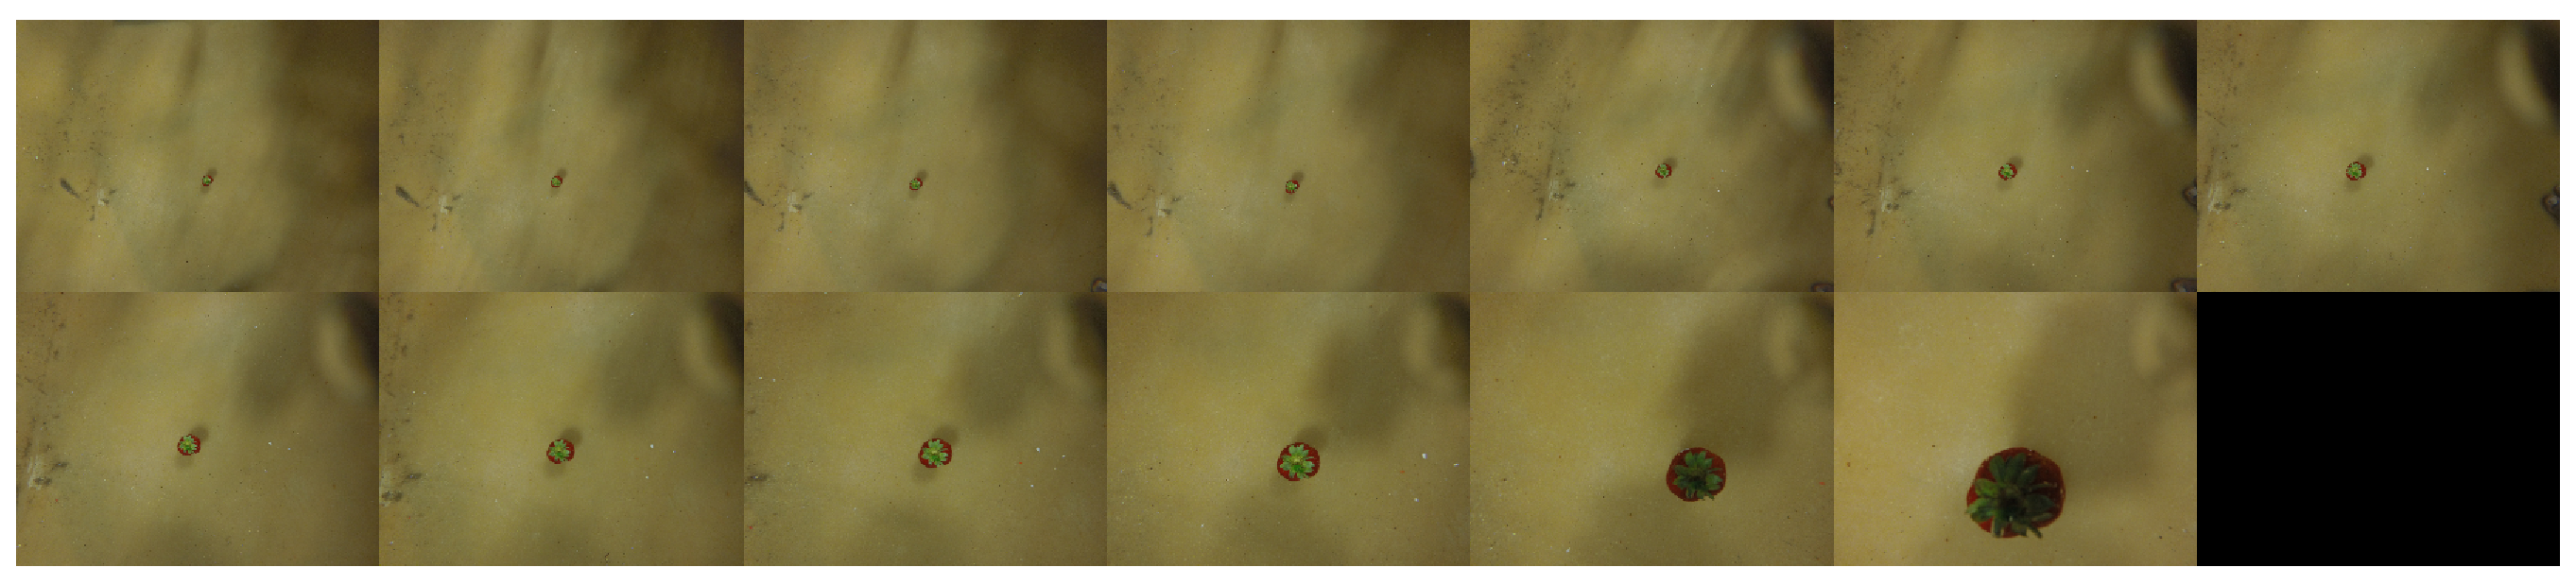
\includegraphics[width=\textwidth]{strawberry_distance_montage.eps}
      \caption{Strawberry specimen seen from different heights}
      \label{fig:strawberry_height_specimen}
  \end{subfigure}
  \begin{subfigure}[]{\textwidth}
      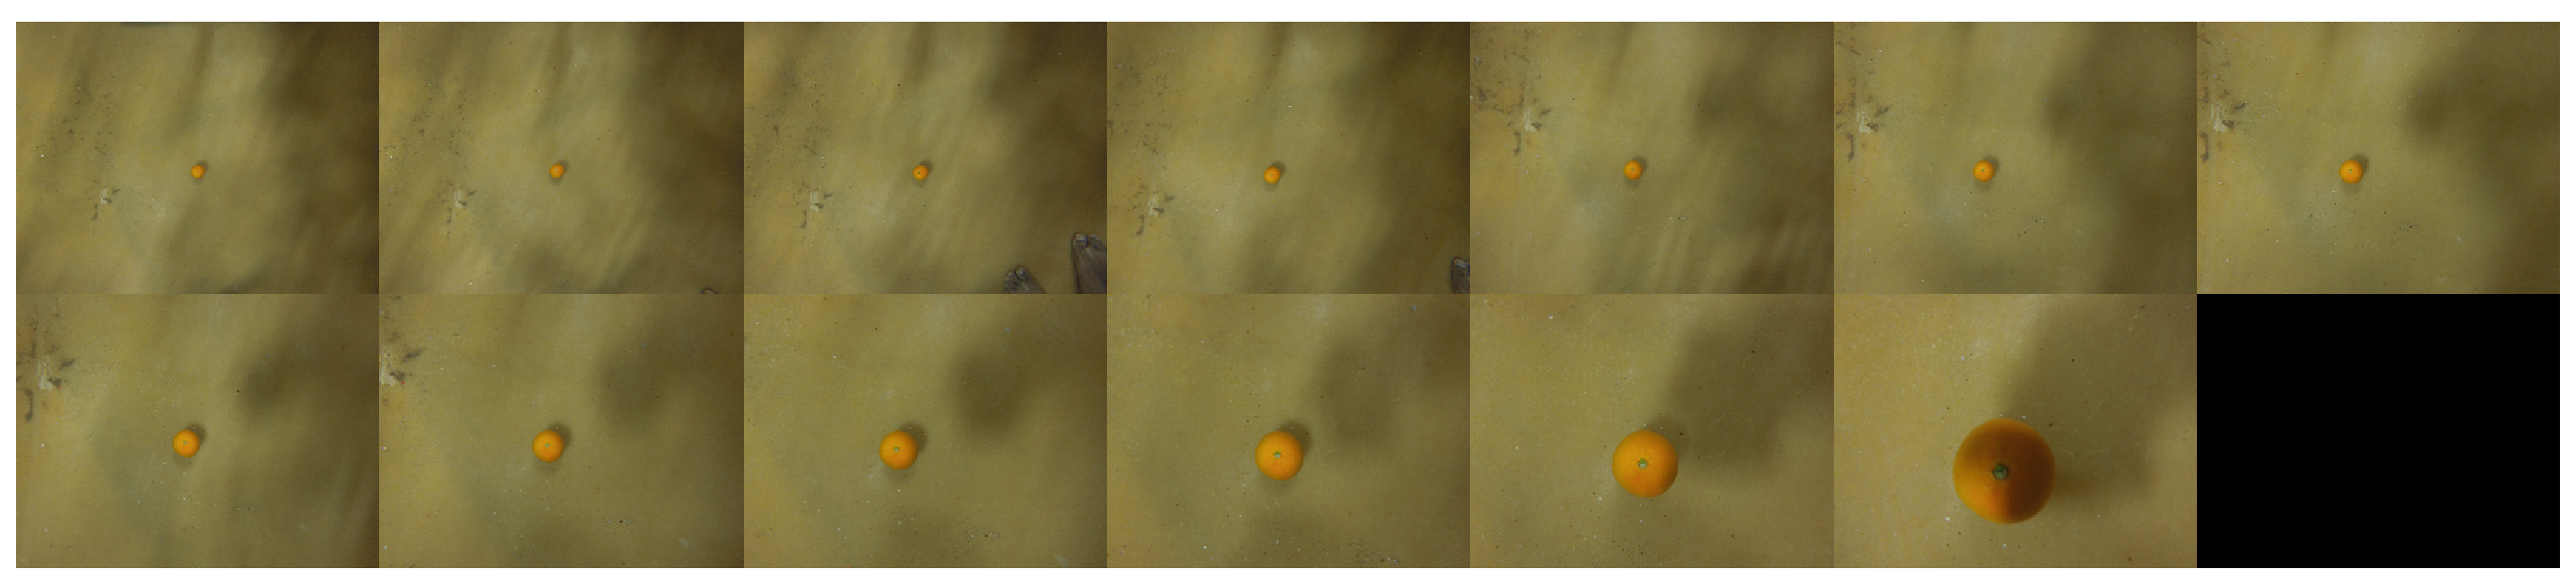
\includegraphics[width=\textwidth]{orange_distance_montage.eps}
      \caption{Orange specimen seen from different heights}
      \label{fig:orange_height_specimen}
  \end{subfigure}
\caption[Set of images collected for each specimen from different heights]{A set of 13 images gathered for a specimen (strawberry in Figure~\subref{fig:strawberry_height_specimen} and orange in Figure~\subref{fig:orange_height_specimen}) starting from a height of 32 inches (top left) up to a height of 8 inches (bottom right) away from the target.
Each subsequent image was captured 2 inches closer to the specimen}.
\label{fig:height_specimen}
\end{figure*}	
%
Due to the wide-angle fish-eye lens in the GoPro camera used, the ratio of the pixels of the object specimen to the background could be very small when the camera is far away from the target. In technical terms, when the images of a target are captured by a camera that is far away from the specimen, the number of pixels that correspond to the specimen in the image could be statistically insignificant. This object recognition procedure depends on histograms of images (more details of how the histogram is relevant is explained in Section~\ref{sec:distdes_methodology}). 
For the histogram to accurately capture the properties of a specimen, the images of the specimen need to have a high ratio of object pixels over background pixels. To improve the ratio of object pixels in the image, the images were cropped to discard the excess background. The strawberry and orange specimen shown in Figure~\ref{fig:strawberry_height_specimen} and Figure~\ref{fig:orange_height_specimen} are shown again in Figure~\ref{fig:strawberry_height_specimen_cropped} and 
Figure~\ref{fig:orange_height_specimen_cropped} respectively, but after cropping of the excess background.

\begin{figure*}
  \centering
  \begin{subfigure}[]{0.12\textwidth}
      \includegraphics[width=\textwidth]{strawberry4_obj_01/strawberry4_001_32}
      \caption{}
  \end{subfigure}
  \begin{subfigure}[]{0.12\textwidth}
      \includegraphics[width=\textwidth]{strawberry4_obj_01/strawberry4_001_30}
      \caption{}
  \end{subfigure}
  \begin{subfigure}[]{0.12\textwidth}
      \includegraphics[width=\textwidth]{strawberry4_obj_01/strawberry4_001_28}
      \caption{}
  \end{subfigure}
  \begin{subfigure}[]{0.12\textwidth}
      \includegraphics[width=\textwidth]{strawberry4_obj_01/strawberry4_001_26}
      \caption{}
  \end{subfigure}
  \begin{subfigure}[]{0.12\textwidth}
      \includegraphics[width=\textwidth]{strawberry4_obj_01/strawberry4_001_24}
      \caption{}
  \end{subfigure}
  \begin{subfigure}[]{0.12\textwidth}
      \includegraphics[width=\textwidth]{strawberry4_obj_01/strawberry4_001_22}
      \caption{}
  \end{subfigure}
  \begin{subfigure}[]{0.12\textwidth}
      \includegraphics[width=\textwidth]{strawberry4_obj_01/strawberry4_001_20}
      \caption{}
  \end{subfigure}
  \begin{subfigure}[]{0.12\textwidth}
      \includegraphics[width=\textwidth]{strawberry4_obj_01/strawberry4_001_18}
      \caption{}
  \end{subfigure}
  \begin{subfigure}[]{0.12\textwidth}
      \includegraphics[width=\textwidth]{strawberry4_obj_01/strawberry4_001_16}
      \caption{}
  \end{subfigure}
  \begin{subfigure}[]{0.12\textwidth}
      \includegraphics[width=\textwidth]{strawberry4_obj_01/strawberry4_001_14}
      \caption{}
  \end{subfigure}
  \begin{subfigure}[]{0.12\textwidth}
      \includegraphics[width=\textwidth]{strawberry4_obj_01/strawberry4_001_12}
      \caption{}
  \end{subfigure}
  \begin{subfigure}[]{0.12\textwidth}
      \includegraphics[width=\textwidth]{strawberry4_obj_01/strawberry4_001_10}
      \caption{}
  \end{subfigure}
  \begin{subfigure}[]{0.12\textwidth}
      \includegraphics[width=\textwidth]{strawberry4_obj_01/strawberry4_001_08}
      \caption{}
  \end{subfigure}
\caption[Images of a strawberry specimen after cropping excess background]{The strawberry specimen in Figure~\ref{fig:strawberry_height_specimen} after cropping to remove excess background}
\label{fig:strawberry_height_specimen_cropped}
\end{figure*}	

\begin{figure*}
  \centering
  \begin{subfigure}[]{0.12\textwidth}
      \includegraphics[width=\textwidth]{orange4_obj_11/orange4_011_32}
      \caption{}
  \end{subfigure}
  \begin{subfigure}[]{0.12\textwidth}
      \includegraphics[width=\textwidth]{orange4_obj_11/orange4_011_30}
      \caption{}
  \end{subfigure}
  \begin{subfigure}[]{0.12\textwidth}
      \includegraphics[width=\textwidth]{orange4_obj_11/orange4_011_28}
      \caption{}
  \end{subfigure}
  \begin{subfigure}[]{0.12\textwidth}
      \includegraphics[width=\textwidth]{orange4_obj_11/orange4_011_26}
      \caption{}
  \end{subfigure}
  \begin{subfigure}[]{0.12\textwidth}
      \includegraphics[width=\textwidth]{orange4_obj_11/orange4_011_24}
      \caption{}
  \end{subfigure}
  \begin{subfigure}[]{0.12\textwidth}
      \includegraphics[width=\textwidth]{orange4_obj_11/orange4_011_22}
      \caption{}
  \end{subfigure}
  \begin{subfigure}[]{0.12\textwidth}
      \includegraphics[width=\textwidth]{orange4_obj_11/orange4_011_20}
      \caption{}
  \end{subfigure}
  \begin{subfigure}[]{0.12\textwidth}
      \includegraphics[width=\textwidth]{orange4_obj_11/orange4_011_18}
      \caption{}
  \end{subfigure}
  \begin{subfigure}[]{0.12\textwidth}
      \includegraphics[width=\textwidth]{orange4_obj_11/orange4_011_16}
      \caption{}
  \end{subfigure}
  \begin{subfigure}[]{0.12\textwidth}
      \includegraphics[width=\textwidth]{orange4_obj_11/orange4_011_14}
      \caption{}
  \end{subfigure}
  \begin{subfigure}[]{0.12\textwidth}
      \includegraphics[width=\textwidth]{orange4_obj_11/orange4_011_12}
      \caption{}
  \end{subfigure}
  \begin{subfigure}[]{0.12\textwidth}
      \includegraphics[width=\textwidth]{orange4_obj_11/orange4_011_10}
      \caption{}
  \end{subfigure}
  \begin{subfigure}[]{0.12\textwidth}
      \includegraphics[width=\textwidth]{orange4_obj_11/orange4_011_08}
      \caption{}
  \end{subfigure}
\caption[Images of an orange specimen after cropping excess background]{The orange specimen in Figure~\ref{fig:orange_height_specimen} after cropping to remove excess background}
\label{fig:orange_height_specimen_cropped}
\end{figure*}	


\subsection{Annotation Process}
\label{sec:distdes_annotation}

Just like any other supervised machine learning algorithm, this method requires annotation of images into labeled background and foreground. The task of annotation is a costly and labor intensive process. The whole idea of developing an object recognition algorithm is often related to avoiding human annotation or any other form of manual intervention to identify objects from images. However, to accomplish this task an initial set of images need to be annotated manually to contribute to the learning set of a machine learning algorithm. In this object recognition method, each learning sample constitutes 13 images of a specimen from different heights. This increases the task of annotation 13-fold. To avoid or at least minimize the manual annotation involved, a semi-automated annotation framework was devised.

In the first stage of the annotation process, \gls{buva} technique (described in Section~\ref{sec:visual_attn}) is used to pick the most \textit{interesting} point in an image. According to the visual attention hypothesis, if a distribution of features can be used to characterize an image, the most interesting point or the first fixation corresponds to the point in the image which is most unlikely to belong to the distribution of features of the image. In other words, the first fixation corresponds to a point that does not belong to the background and hence most likely is a foreground object pixel. In the first stage of this annotation process, the first fixation point along with all its neighboring pixels within a rectangle of dimensions $15\% \,image\, width \times 15\% \,image\, height$ centered on the fixation are assumed to be foreground pixels. We will refer to this rectangle as the \textit{foreground hypothesis rectangle}.
Since the data collection  process ensures that an object in an image is close to the center of the image rather than the edges of the image, the pixels in the boundary of the images can safely be assumed to be background pixels. Hence, rectangular blocks of pixels in the 4 corners of an image, of dimension $5\% \,image\, width \times 5\% \,image\, height$, are labeled as background seed pixels. The foreground and background pixel hypothesis thus obtained are used in the next stage of the annotation process to segment the image into foreground and background.

The foreground and background seeds obtained before can be used to initialize a grabcut-in-one-cut algorithm \cite{onecut}. This grabcut-in-one-cut algorithm, a variant of graphcut algorithm (described in Section~\ref{sec:onecut}) bifurcates an input image into background and foreground by labeling pixels \textit{similar} in appearance to foreground seeds as foreground and the other pixels that appear closer to background seeds as background. The result of this graphcut algorithm is a binary labeling of an image into foreground and background pixels. 
However, the result from the visual attention process that supplies the foreground seeds might not produce accurate results in all cases. There are often instances when the region tagged as foreground contains edge pixels of an object. This is explained by the nature of visual attention to pick points that constitute indicators of a change in distribution which could easily be points at the edge of an object that are essentially discontinuities indicating a transition between foreground and background pixel distributions. Visual attention picking object edge pixels could result in the foreground seeds inside foreground hypothesis rectangle erroneously containing some background pixels. An illustration of this effect can be seen in Figure~\ref{fig:good_seg_visualattn_seeds} where the green dot at the edge of the object is the determined visual attention fixation. The blue foreground hypothesis rectangle around the fixation point contains some wrongly labeled background pixels provided as input foreground 
pixels to the graphcut algorithm. Background pixels in the foreground seeds provided to the graphcut segmentation algorithm can result in inaccurate segmentation as seen in Figure~\ref{fig:good_seg_visualattn_seg}. Thus to improve the performance of the graphcut algorithm, we use a process to iteratively refine the foreground seeds. This task of iterative refinement operates by taking the result of the graphcut segmentation obtained through the foreground seeds from visual attention and computing the centroid of the foreground pixels generated after the application of graphcut algorithm. This centroid acts as the new center of the foreground hypothesis rectangle for the next iteration of graphcut segmentation. This process is repeated till the segmentation results stabilize. In other words, this iterative graphcut process is repeated 
till the number of foreground pixels from the previous iteration rejected as background by the current iteration is within a small threshold of 5\%. In mathematical terms, if $F_i$ is the set of foreground pixels labeled by the graphcut algorithm in iteration $i$, then the iterative process is continued till the condition in \eqref{eqn:seg_threshold} is met. The change in the blue foreground hypothesis rectangle after recursive graphcut segmentation and the resulting improved foreground labeling can be seen in Figure~\ref{fig:good_seg_recursive_seeds} and Figure~\ref{fig:good_seg_recursive_seg} respectively.
%
\begin{equation}
 \label{eqn:seg_threshold}
 \frac{|F_{i-1}-F_{i}|}{|F_i|} \leq 0.05
\end{equation}
%
%
\begin{figure*}
  \centering
  \begin{subfigure}[]{0.2\textwidth}
      \includegraphics[width=\textwidth]{distdes_annotation_good_visualattn_seeds}
      \caption{}
      \label{fig:good_seg_visualattn_seeds}
  \end{subfigure}
  \begin{subfigure}[]{0.2\textwidth}
      \includegraphics[width=\textwidth]{distdes_annotation_good_visualattn_segment}
      \caption{}
      \label{fig:good_seg_visualattn_seg}
  \end{subfigure}
  \begin{subfigure}[]{0.2\textwidth}
      \includegraphics[width=\textwidth]{distdes_annotation_good_recursive_seeds}
      \caption{}
      \label{fig:good_seg_recursive_seeds}
  \end{subfigure}
  \begin{subfigure}[]{0.2\textwidth}
      \includegraphics[width=\textwidth]{distdes_annotation_good_recursive_segment}
      \caption{}
      \label{fig:good_seg_recursive_seg}
  \end{subfigure}
\caption[Illustration of annotation process flow]{A graphical illustration of operation of visual attention and recursive graphcut as a part of the annotation process flow is shown here. Figure~\subref{fig:good_seg_visualattn_seeds} shows the visual attention fixation as a green dot. Since the visual attention fixation is on the edge of the object, the foreground hypothesis rectangle shown in blue contains background pixels. When the graphcut algorithm operates on Figure~\subref{fig:good_seg_visualattn_seeds} utilizing the pixels inside the blue rectangle as the foreground seeds and the pixels inside the red rectangles in the corners of the image as background seeds, the resulting segmented foreground region is displayed in Figure~\subref{fig:good_seg_visualattn_seg}. Due to the presence of background pixels in the input foreground seeds supplied to the graphcut algorithm, the segmentation result obtained in Figure~\subref{fig:good_seg_visualattn_seg} is inaccurate. When recursive graphcut algorithm is 
applied, the blue foreground hypothesis rectangle eventually moves towards the center of the object, as seen in Figure~\subref{fig:good_seg_recursive_seeds}, and no longer contains background pixels. With the updated foreground hypothesis rectangle after recursive graphcut segmentation, the improved segmentation result can be seen in Figure~\subref{fig:good_seg_recursive_seg}}.
\label{fig:annotation_good_seg}
\end{figure*}	
%
When the foreground region labels from the graphcut algorithm stabilize, its unlikely for the foreground region to change with additional iterations. This stabilization condition captured in \eqref{eqn:seg_threshold}, indicates that the foreground region label hypothesis generated by graphcut has converged. In case the convergence condition in \eqref{eqn:seg_threshold} is not met after $N=5$ iterations, further recursion is abandoned and the labeling results available after $N$ iterations is taken.

Though this process appears to be fully automated, there are cases where this automated segmentation fails. A case of segmentation failure could be due to foreground seeds identified by visual attention not belonging to the specimen in the image. Visual attention not picking up the specimen could be due to the presence of other \emph{interesting} artifacts in the image that bias visual attention away from the specimen. There are also cases where the texture of the specimen is not uniform, in which case visual attention could be biased towards a specific part of the object. This could result in graphcut segmentation only identifying the sub-region of the specimen that biased the visual attention fixation. An instance of only segmenting a sub-region of the specimen is often seen in the case of strawberry which is characterized by a green stalk along with a reddish pulp. Visual attention and graphcut could end up mistakenly segmenting either the green stalk or the red pulp only. This case is graphically 
described in Figure~\ref{fig:annotation_bad_seg}. The visual attention fixation shown by a green dot in Figure~\ref{fig:bad_seg_visualattn_seeds} is biased towards the green stalk region of the strawberry specimen. An application of recursive graphcut on this example only ends up segmenting the green stalk region as seen in Figure~\ref{fig:bad_seg_recursive_seg}. Such cases of failure of automated annotation process are rectified here through human verification and inclusion of foreground seeds that are representative of the complete specimen, i.e. both the green stalk and the red pulp sub-regions of strawberry in this case. Therefore, to prevent failed cases of segmentation degrading the learning set, a manual verification process is added as the last step of this annotation process. During this process, for all failed instances of automated segmentation, the foreground and background seed pixels are manually set. 
%
\begin{figure*}
  \centering
  \begin{subfigure}[]{0.2\textwidth}
      \includegraphics[width=\textwidth]{distdes_annotation_bad_visualattn_seeds}
      \caption{}
      \label{fig:bad_seg_visualattn_seeds}
  \end{subfigure}
  \begin{subfigure}[]{0.2\textwidth}
      \includegraphics[width=\textwidth]{distdes_annotation_bad_recursive_segment}
      \caption{}
      \label{fig:bad_seg_recursive_seg}
  \end{subfigure}
\caption[Illustration of failed automated annotation process flow]{A graphical illustration of a failure case of automated annotation process which requires human verification and correction. The visual attention fixation shown as a green dot in Figure~\subref{fig:good_seg_visualattn_seeds} is biased towards the green stalk region of the strawberry. Since this strawberry specimen exhibits binary texture--green stalk and red pulp, the combined visual attention and graphcut automated annotation approach ends up segmenting only the stalk sub-region of this strawberry specimen as the foreground, as portrayed in Figure~\subref{fig:bad_seg_recursive_seg}. Such cases of failure of the automated annotation approach calls for human verification and correction of foreground seeds to enable graphcut algorithm to segment the whole strawberry specimen}. 
\label{fig:annotation_bad_seg}
\end{figure*}	
%

This final manual verification and correction process requires human effort. However, during experiments it was noted that a very small percentage of cases needed corrective action. In summary, this semi-automated annotation process is relatively less cumbersome than a fully manual annotation effort. An illustration of the output of the annotation process for a single specimen is shown in Figure~\ref{fig:orange_segment_height_montage}. Figure~\ref{fig:orange_segment_height_montage} represents a montage of 13 images of an orange specimen with the top-left component showing the segmented foreground from the image captured 32 inches away from the orange specimen. Likewise the bottom-most row shows the image that was captured 8 inches away from the specimen. The montage in Figure~\ref{fig:orange_segment_height_montage} is arranged such that the 13 images, from left to right, are in the decreasing order of the heights from which the images were capture. This sequence of images in the montage wraps around after 
every 4 images resulting in four rows to represent 13 images.
%
\begin{figure*}
  \centering
  \includegraphics[width=\textwidth]{orange_height_segment_montage}
  \caption[Annotation output for a single specimen]{The output of the annotation process showing a montage of the foreground segmented from a set of 13 images that belong to a single orange specimen. The left-top montage component is the image of the orange specimen captured 32 inches from the ground. The montage components arranged from left to right to progressively show images that were captured closer to the orange specimen. The closest image that was captured is 8 inches away from the specimen and is shown in the bottom-most row.} 
  \label{fig:orange_segment_height_montage}
\end{figure*}	
%


\subsection{Learning}

\begin{enumerate}
	\item Learning phase of a machine learning method involves parsing labeled data to identify features that can reliably indicate the identity of an object.
	
	\item In this method, we extract features from multiple images of a target acquired from different heights.
	
	\item Manual intervention is minimized by using visual attention to aid the detection of interesting regions in the image that could be targets.
	
	\item Graphcut is then segments the detected interesting regions using the the visual attention fixations as foreground seeds.
	
	\item In case of failure of this automated detection and segmentation approach seeds are selected manually for the graphcut algorithm to operate on.
	
	\item A histogram based distance metric is used to compare the images with segmented object and the unsegmented image corresponding to each of the 13 samples available for each target object.
	
	\item The information available from the histogram distance metric for data collected from different heights is used to construct a single feature descriptor for each instance of the target.
	
	\item The feature descriptor from all target instances are then combined to produce a feature distribution for the target.
\end{enumerate}


The learning phase of a machine learning based object recognition method involves identifying patterns in the data that represent the presence of an object. The annotated information fed to the algorithm is a pre-specified labeling of the data into foreground and background. The responsibility of the learning method here is to identify patterns in designated foreground regions, meanwhile also using information from labeled background to reject false positives. The learning algorithm then uses the patterns it identifies from the annotated foreground and background pixels to generate a learned model that is capable of identifying foreground pixels from an image.

In the machine learning technique developed in this paper, instead of using individual images with annotations of foreground and background a collection of 13 images each featuring the same specimen from a known height is utilized. This adds an additional height dimension to the feature space. The driving goal here is to encode the variation in appearance of a specimen from different heights to build a robust object recognition classifier. Height here offers an additional dimension in the feature space for the learning algorithm to capitalize on.

Since this object recognition algorithm is positioned to operate on images without prior segmentation. The features used in this algorithm should be sufficiently generic to capture the appearance of an object directly from an image without foreground segmentation. To achieve this, we use the histogram signatures (described in Section~\ref{sec:hist_signature}) to extract information from an image in HSI-colorspace. This information from multiple specimens belonging to the same object class is then combined to generate a feature distribution. The details of this process is described in the rest of this section.

\subsubsection{Feature Distribution}
\label{sec:distdes_feature_distr}

The first part of the feature distribution generation process is the computation of the hue, saturation and intensity histogram signatures on the labeled foreground pixels only in the learning dataset. The parameters chosen for the histogram signature computation: the number of equally spaced bins in the histogram $|\mathcal{B}|=256$ and the upper bound on the number of pixels affected by noise $e=5\%$. Using these parameters the histogram signatures for all three components of the HSI-colorspace (hue, saturation and intensity) is calculated on all 13 height-tagged images of a specimen, only on the labeled foreground pixels in the image. Lets represent the histogram signature of the labeled foreground for specimen $k$ with height tag $h$ belonging to class $c$ as on the color component $f=\{H \text{ hue}, S \text{ saturation}, I \text{ intensity}\}$ be represented as $\mathcal{H}^{c_{hk}}_f$. Since there are 3 color components, we realize 3 histogram signatures per height-tagged image of a specimen. If we 
consider all the 13 height-tagged images available for a specimen, the total histogram signatures now available is 39 ($13 \times 3$).

In the next stage of the learning process, the histogram signatures $\mathcal{H}^{c_{hk}}_f$ from all specimens belonging to a single object class are combined to generate a generalized histogram signature for the object class.
In order to achieve this, the mean of all histogram signatures corresponding to a specific height-tag from all specimens of a class are combined. In other words, the mean $\bar{\mathcal{H}}^{c_{h}}_f$ of all histogram signatures with  height-tag $h$ are computed by taking the mean of individual components of the $256$-D vectors of sequence of histogram signatures $\mathcal{H}^{c_{h1}}_f, \mathcal{H}^{c_{h2}}_f, \mathcal{H}^{c_{h3}}_f, \ldots, \mathcal{H}^{c_{hm}}_f$, where $m$ is the number of specimens of class $c$ available in the learning dataset. Mathematically speaking the computation of the $j$-th component of the $256$-D mean histogram $\bar{\mathcal{H}}^{c_{h}}_f$ is given as
\begin{align}
 \left[\bar{\mathcal{H}}^{c_{h}}_f\right]_j=\sum_{k=1}^{m} \left[ \mathcal{H}^{c_{hk}}_f \right]_j.
\end{align}
Since there are 13 different height-tags from which data was collected along with 3 different color components, each object class $c$ is represented by a sequence of $39\, (13 \times 3)$ histogram signatures which will be collectively referred to as $\bar{\mathcal{H}}^{c}$.

The sequence of $39$ histogram signatures $\bar{\mathcal{H}}^{c}$ captures the generalized appearance of the objects of class $c$. Its important to note that the data used to compute this generalized histogram signature is composed of foreground pixels of object specimens only without any background information. If we are to use such a generalized histogram signature generated only from foreground information for classifying objects, it will necessitate prior processing of an image to detect and segment objects present in the images before this generalized histogram signature $\bar{\mathcal{H}}^{c}$ can be used for classification purposes. However one of the goals of this paper is to avoid segmentation while attempting classification of objects from images. To achieve this, we revisit the learning dataset to use the background information and build a representation that captures how inclusion of background pixels to different individual histogram signatures affects the generalized histogram signature $\bar{\
mathcal{H}}^{c}$ of class $c$. 

In order to use background information for building a classified we first generate another set of histogram signatures.
For specimen $k$ of class $c$ from the learning dataset, we compute a sequence of $39$ histogram signatures similar to the computation involved in $\mathcal{H}^{c_{hk}}_f$ but now utilizing all pixels in the image instead of just the foreground pixels. This set of 39 histograms $\ddot{\mathcal{H}}^{c_{k}}$ for specimen $k$ of class $c$ is given by
\begin{align}	\label{eqn:hist_signature}
 \ddot{\mathcal{H}}^{c_{k}} = \ddot{\mathcal{H}}^{c_{hk}}_f \Big|_{h\times f},
\end{align}
%
where $h=\{8,10,12, \ldots,32\}$ and $f=\{H,S,I\}$.

Once we have the sequence of histogram signatures $\ddot{\mathcal{H}}^{c_{k}}$ of specimen $k$ belonging to class $c$ along with the generalized histogram signature $\bar{\mathcal{H}}^{c}$ of class $c$, a numeric distance measure $D$ between the histogram signatures can be computed. If we have a series of such distance measures evaluated for a collection of specimens of class $c$, a distribution of these distance measures can be generated. This distribution 
of distance measures encodes the variability in generalized histogram signature $\bar{\mathcal{H}}^{c}$ induced by the presence of background pixels along with foreground pixels. In effect this offers an avenue to check images for the presence of an object of class $c$ without any prior segmentation of foreground pixels. The distance measure in  \eqref{eqn:hist_signature_dist} used for this purpose is the \emph{$L_2$-norm} between two vectors.
%
\begin{align}	\label{eqn:hist_signature_dist}
 d_{chfk} = D(\bar{\mathcal{H}}^{c_{hk}}_f, \ddot{\mathcal{H}}^{c_{hk}}_f) 
 = \sqrt{\sum_{j=1}^{|B|}\Bigg(\left[\bar{\mathcal{H}}^{c_{hk}}_f\right]_j
 -\left[\ddot{\mathcal{H}}^{c_{hk}}_f\right]_j\Bigg)^2}
\end{align}

Since there are 39 histograms in total, we also get a sequence of 39 $d_{chfk}$ values for the $k$-th specimen of class $c$ which will be represented as $d_{ck}$,
%
\begin{align}	\label{eqn:dist_sequence}
 d_{ck}=d_{chf}\Big|_{h\times f}\,,
\end{align}
%
where $h=\{8,10,12, \ldots,32\}$ and $f=\{H,S,I\}$.

A sequence of distance measures $d_{ck}$ for each specimen $k$ among the $m$ specimens of class $c$ provides a representation of a feature vector of size 39 that describes the appearance of an image that contains a specimen of class $c$. If we consider the feature vectors of all the $m$ available specimens $d_{c1},d_{c2},\ldots,d_{cm}$, a feature distribution sequence $F_c$ that represents the appearance of images containing objects of class $c$ can be formulated. Lets assume that the $m$ values $d_{chf1}, d_{chf2},\ldots,d_{chfm}$ are drawn from a normal distribution 
%
\begin{align}
 F_{chf}\sim &\mathcal{N}(\mu_{chf},\sigma^2_{chf})\label{eqn:normal_distr}\\
 \mu_{chf}= &\frac{\sum_{k=1}^m d_{chfk}}{m}\label{eqn:normal_mean}\\
 \sigma^2_{chf}= &\frac{\sum_{k=1}^m (d_{chfk}-\mu_{chf})^2}{m-1}\label{eqn:normal_stddev}.
\end{align}
%
Then the feature distribution sequence $F_c$ can be represented as a sequence of 39 distributions,
\begin{align}	\label{eqn:feat_distribution}
 F_c=F_{chf}\Big|_{h \times f}
\end{align}
where $h=\{1,2,\ldots,13\}$ and $f=\{H,S,I\}$. 

For the two classes of objects, Strawberry with 13 specimens and Orange with 11 specimens, their respective feature distributions $F_s$ and $F_o$ can be computed using the procedure discussed in this section. The feature distributions $F_s$ and $F_o$ are shown in Figure~\ref{fig:feat_distr}. The 39 distributions (see \eqref{eqn:normal_distr}) in the distribution sequence are shown along the $x$-axis. Each distribution here is represented by a dot and a bar adjoining it. The dot corresponds the mean and bar corresponds to the 95\% confidence interval or the $2\sigma$ standard deviation interval of the distribution shown in \eqref{eqn:normal_distr}.
%
\begin{figure*}
  \centering
  \begin{subfigure}[]{0.8\textwidth}
      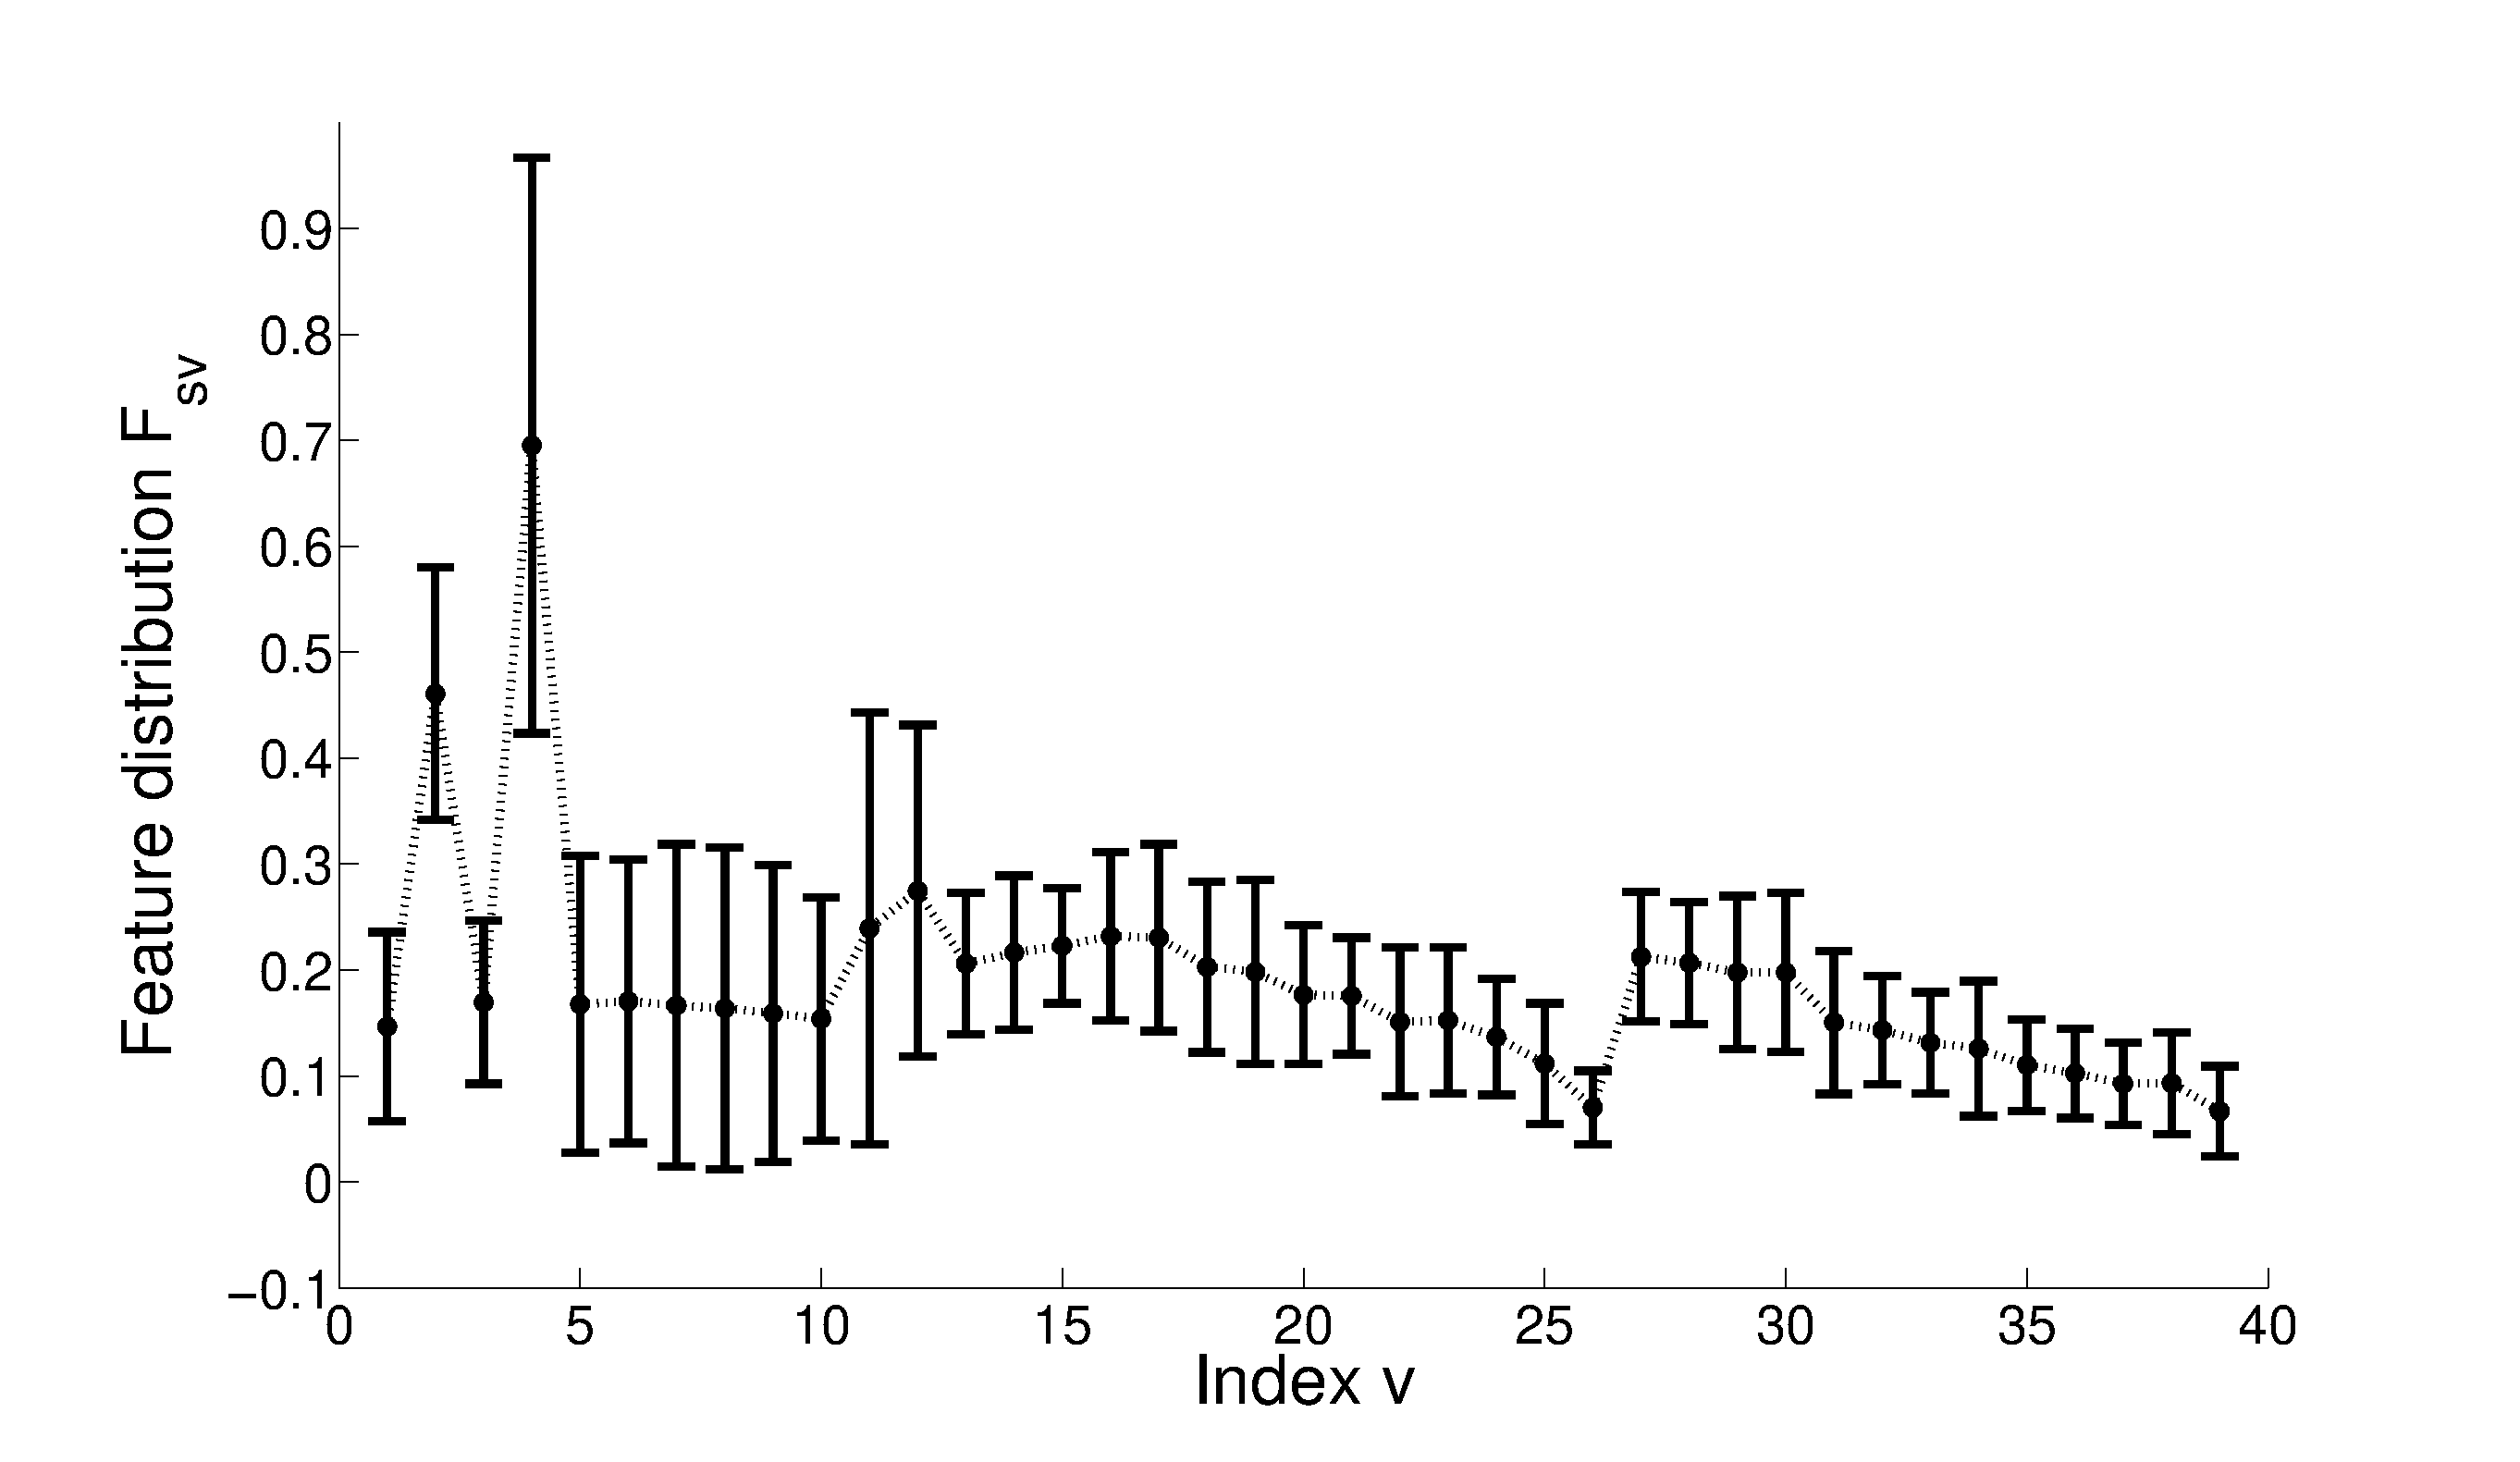
\includegraphics[width=\textwidth]{strawberry_learning_feature_distribution}
      \caption{}
      \label{fig:feat_distr_strawberry}
  \end{subfigure}
  \begin{subfigure}[]{0.8\textwidth}
      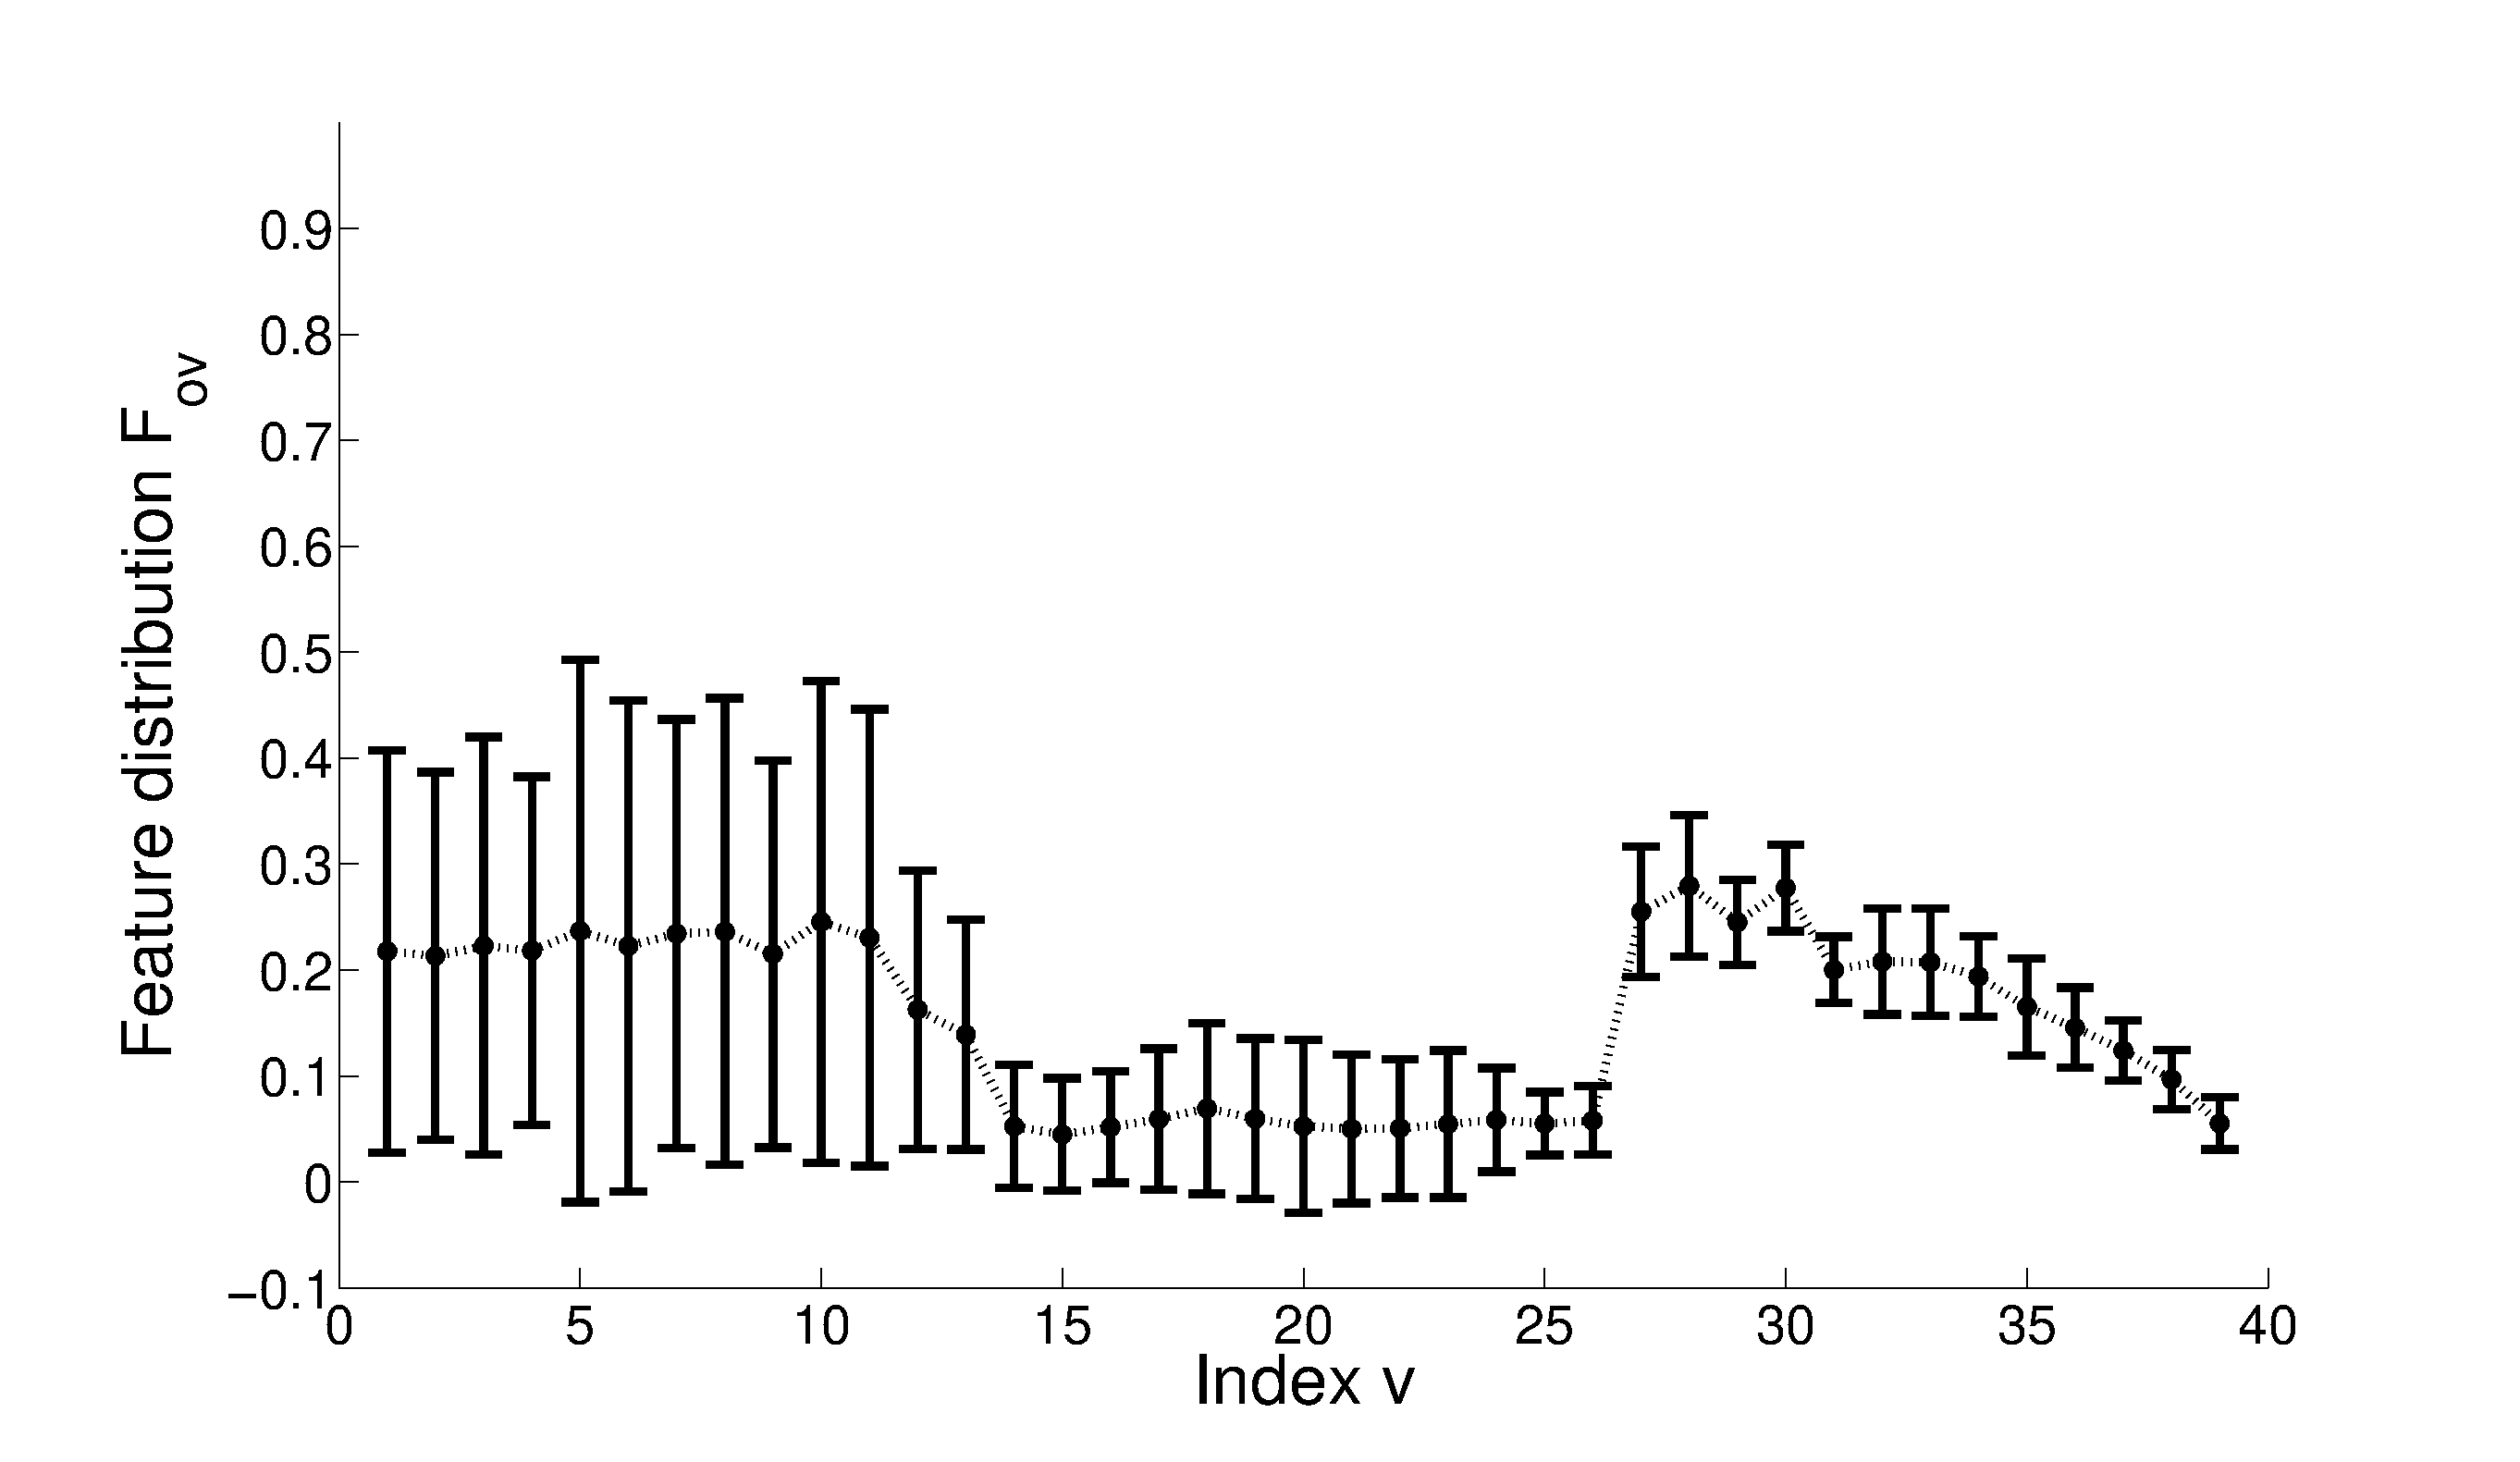
\includegraphics[width=\textwidth]{orange_learning_feature_distribution}
      \caption{}
      \label{fig:feat_distr_orange}
  \end{subfigure}
\caption[Feature distribution]{Strawberry feature distribution sequence $F_s$ and Orange feature distribution sequence $F_o$ generated from 13 strawberry specimens and 11 orange specimens are shown in \subref{fig:feat_distr_strawberry} and \subref{fig:feat_distr_orange} respectively. The $x$-axis corresponds to the index of the distributions in feature distribution sequence. All 39 distributions \eqref{eqn:normal_distr} are shown along the $x$-axis. The  mean of each distribution (see \eqref{eqn:normal_distr}) shown as a dot along with a bar that corresponds to the 95\% confidence interval is also shown.}
\label{fig:feat_distr}
\end{figure*}	
%

This feature distribution $F_c$ which comprises a sequence of 39 distributions offers a way to test for the presence of an object of class $c$ in an image without prior segmentation. In essence the testing for the presence of an object can be broken down into 39 individual hypothesis tests to see if an image containing an object satisfies each of the 39 distributions in $F_c$. Not all of the 39 hypothesis tests might be equally informative-- some of them could be more relevant than others. To this end, a weighting factor $w_{v}$ can be attached to the $v$-th element in feature distribution sequence $F_c$.  The details involved in the computation of these weight factors is described in the Section~\ref{sec:distdes_feat_wts}.

\subsubsection{Feature Weights}
\label{sec:distdes_feat_wts}

The feature weights offer a way to weight each distribution in the feature distribution sequence $F_c$. In case of a binary classification problem between objects of class $p$ and $q$, we choose the feature weights such that the distributions in the sequence with lower intra-class variance and minimal overlap between the distributions of classes $p$ and $q$ are weighted higher than other distributions in the feature distribution sequence. In the rest of this section the formulation of these feature distribution sequence weights is discussed.

For the object class $p$ and $q$, the corresponding feature distribution sequence $F_p$ and $F_q$ are both a sequence of 39 normal distributions. Let the $v$-th component of sequence $F_p$ be $F_{pv}=\mathcal{N}(\mu_{pv},\sigma^2_{pv})$.
The the 95\% confidence interval of $F_{pv}$ is given by
%
\begin{align}	\label{eqn:conf_interval}
C^{0.95}_{F_{pv}}=[\mu_{pv}-2 \times \sigma_{pv},\, \mu_{pv}+2 \times \sigma_{pv}].
\end{align}
%
The weight $w_{pv}$ of the $v$ component of $F_p$ is given by
\begin{align}
 w'_{pv}= & \frac{1}{(1+ |C_{F_{pv}} \cap C_{F_{qv}}| )\times \sigma_{pv}} \label{eq:feat_wt}\\
 w_{pv}= & \frac{w'_{pv}}{\sum_{j} w'_{pj}}, \label{eqn:feat_wt_norm}
\end{align}
where $|C_{F_{pv}} \cap C_{F_{qv}}|$ corresponds to the length of the interval obtained after the intersection of intervals $C_{F_{pv}}$ and $C_{F_{qv}}$. The first term in the denominator of \eqref{eq:feat_wt} penalizes distributions whose confidence intervals share common extents with the other class in this binary classification problem. In other words, this term penalizes distributions in $F_p$ whose confidence intervals overlap with similar  distribution in $F_q$. The second term in the denominator of \eqref{eq:feat_wt} penalizes distributions with high intra-class variance. Ultimately the weights are normalized as shown in \eqref{eqn:feat_wt_norm}. The 39 feature weight sequence thus computed for a class will collectively be referred to as $W_c$. For the binary classification problem, between Strawberry and Orange specimens, the weight factors computed using \eqref{eqn:feat_wt_norm} are shown in the bar plot in Figure~\ref{fig:feat_weights}. The black bars show the Strawberry class weights and the red 
bars whow the corresponding orange class weights.
%
\begin{figure}
  \centering
  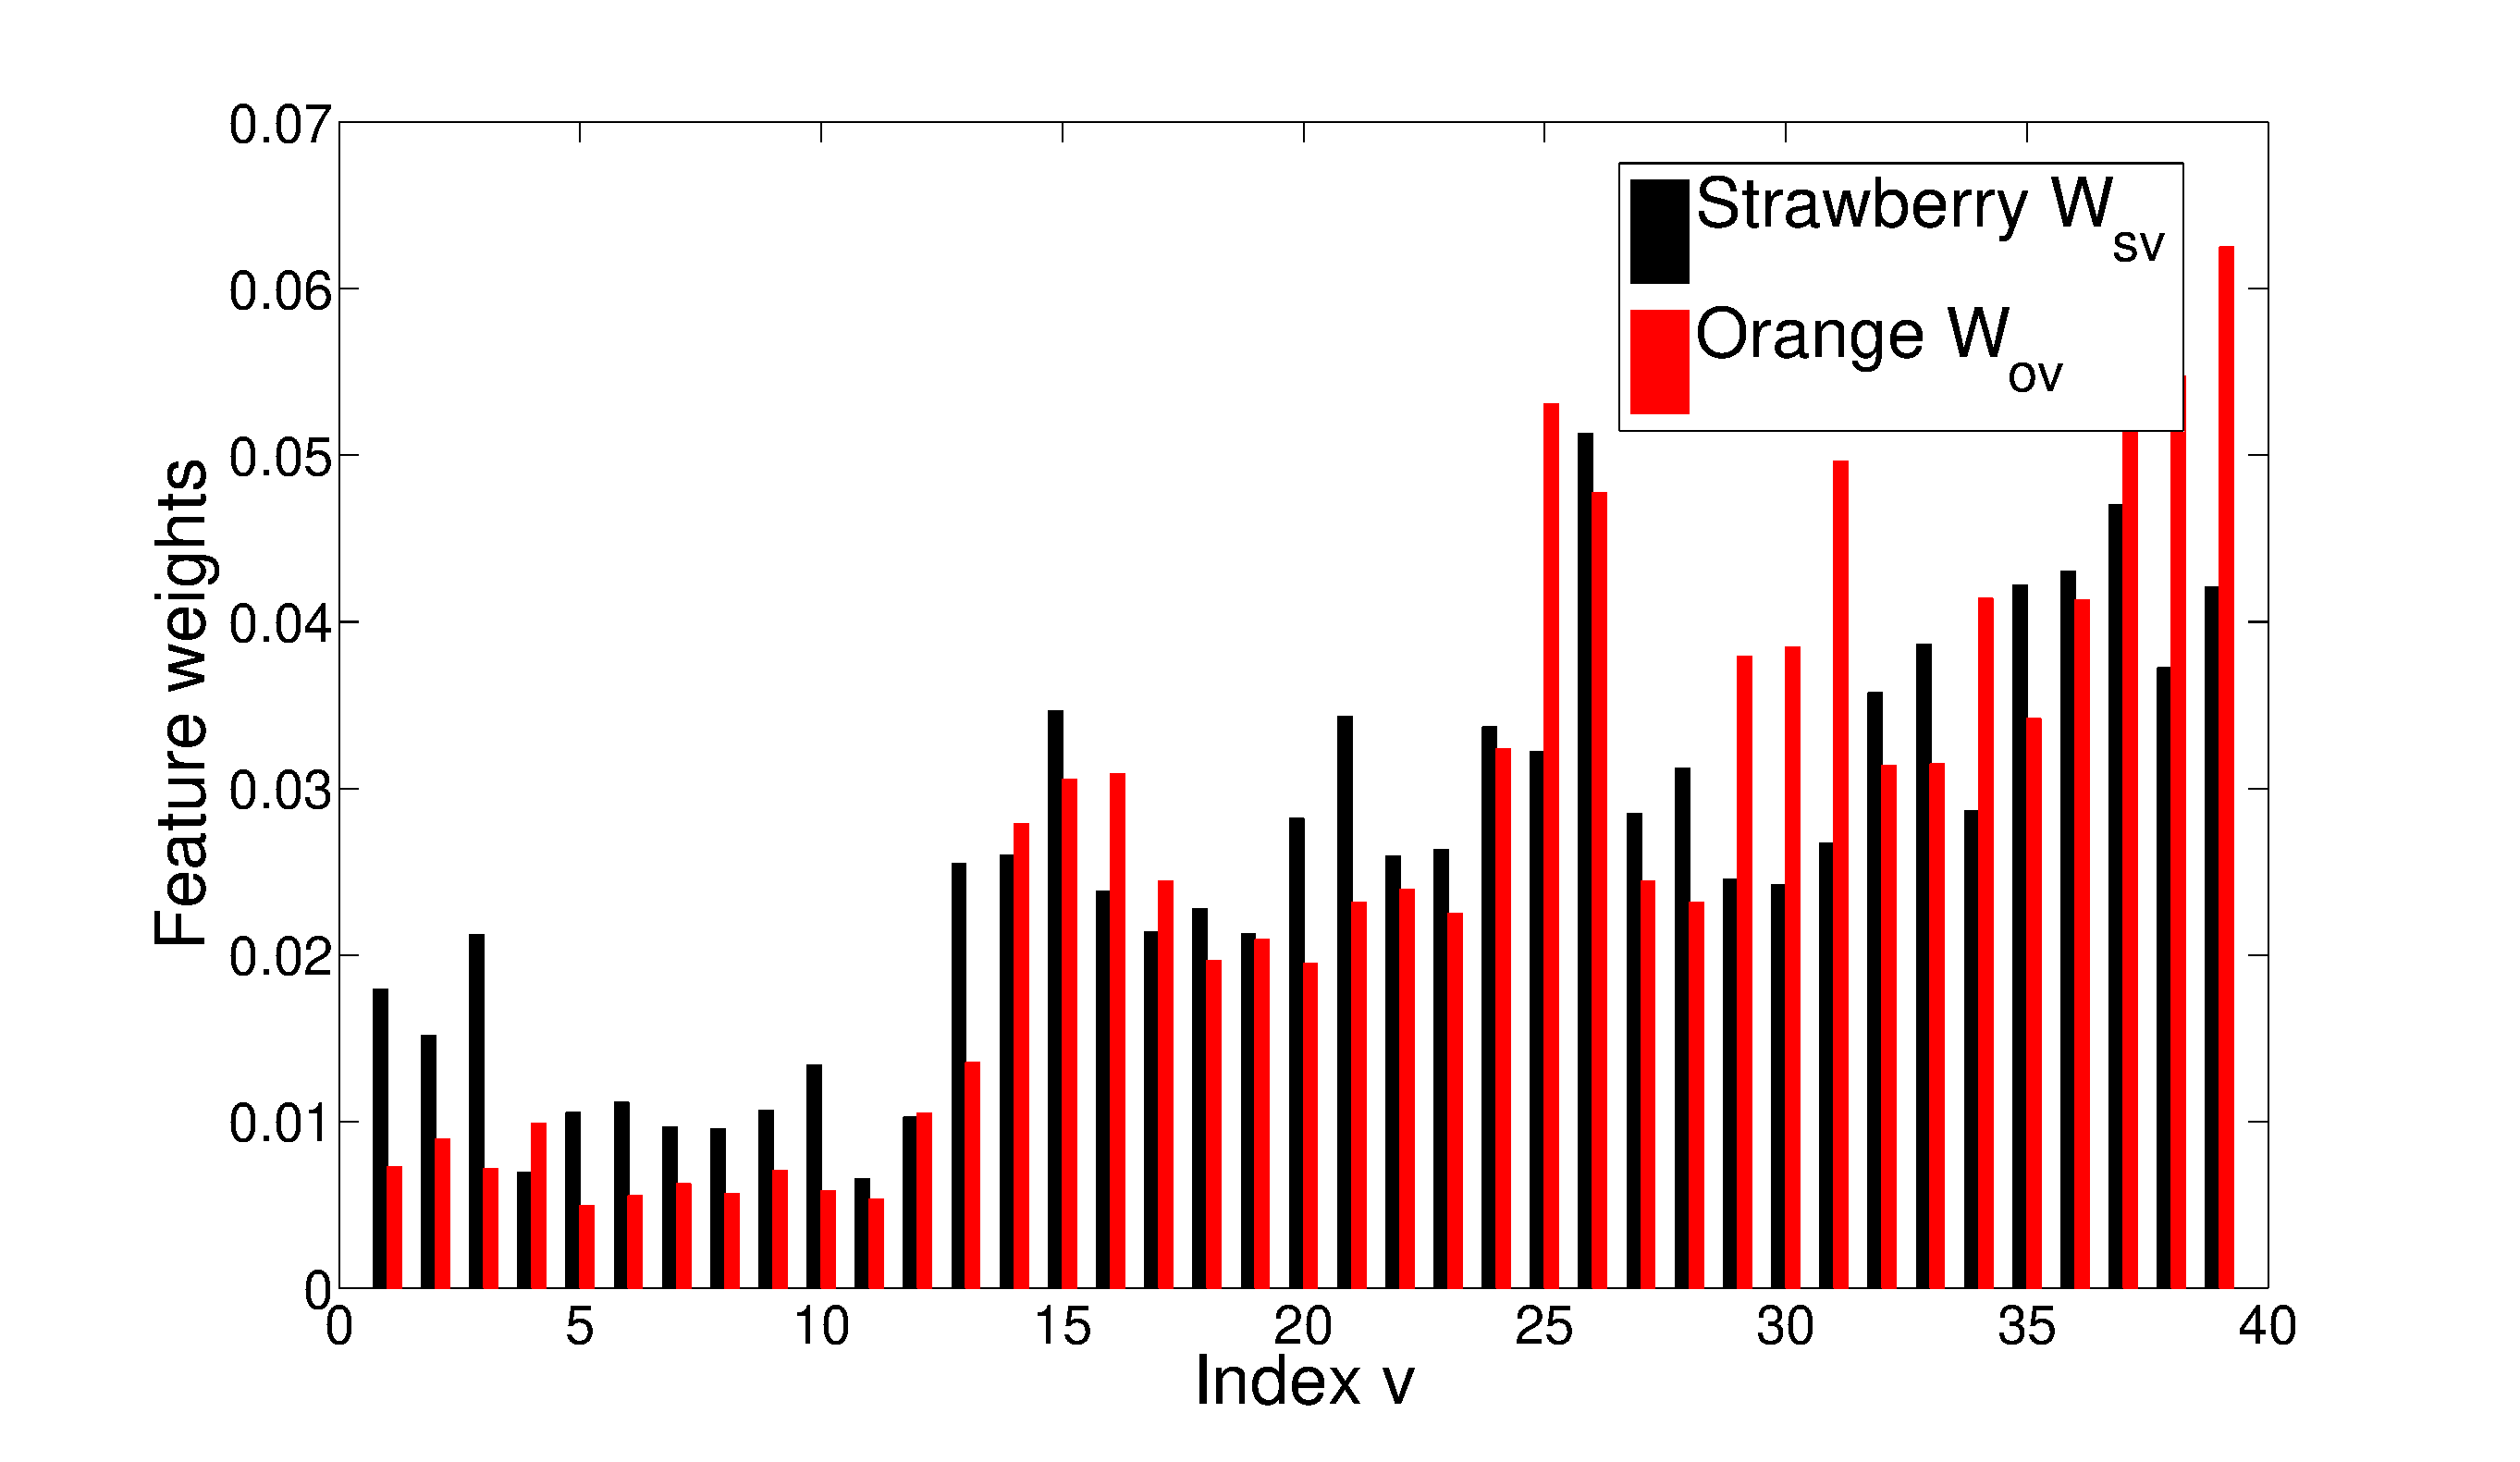
\includegraphics[width=\textwidth]{feature_weights}
  \caption[Feature weights]{The feature weight sequences for Strawberry class $F_s$ and  Orange class $F_o$ are shown as black and red bars respectively.}
  \label{fig:feat_weights}
\end{figure}	
%

The distribution components in $F_p$ with higher values of $w_p$ are weighted higher than the other distributions while performing hypothesis tests that will be discussed in the validation phase of this machine learning algorithm (Section~\ref{sec:distdes_validation}).

\subsection{Validation}
\label{sec:distdes_validation}

\begin{enumerate}
	\item To detect the presence of a target in an image, multiple images of a target are used to compute the feature descriptor.
	
	\item The feature descriptor is then compared against the known classes of feature distributions.
	
	\item If a feature descriptor agrees with a feature distribution for a certain target object class, then the images currently under examination are considered to have sufficient evidence for the presence of an instance from the target object class.
\end{enumerate}

In the object recognition method developed in this paper, a series of height-tagged images of an object specimen can be used to perform a binary classification task and determine the class of the object. In other words, the 13 images of 13 height-tagged images will be used to decide if the object belongs to one of the two classes $p$ and $q$. In order to achieve this, the histogram signatures (described in Section~\ref{sec:hist_signature}) are computed on each of the 13 height tagged-images available for an object specimen. Note the full image is used here as we do not have any pre-specified label information. The computation performed is identical to the one in \eqref{eqn:hist_signature} that results in a sequence of 39 histogram signatures $\ddot{\mathcal{H}}^{k}$. 

The next step in the validation procedure is computing the distance measure in \eqref{eqn:hist_signature_dist} between $\ddot{\mathcal{H}}^{k}$ and the generalized histogram signatures $\bar{\mathcal{H}}^{p}$ and $\bar{\mathcal{H}}^{q}$ of class $p$ and $q$ respectively. This results in 2 sequences of 39 distance values, $D^p_k$ against class $p$ and $D^q_k$ against class $q$, the computation of each of this sequence is identical to \eqref{eqn:dist_sequence}. The sequences $D^p_k$ and $D^q_k$ provide information about the \emph{closeness} of the sample specimen $k$ to each of the classes $p$ and $q$. The information in these sequences need to be further distilled down to eventually attribute specimen $k$ to either class $p$ or class $q$.

Lets assume that specimen $k$ belongs to class $p$. According to this hypothesis, the $v$-th component of $D^p_k$ should satisfy the $v$-th distibution of the feature distribution sequence $F_p$. In other words, using \eqref{eqn:conf_interval}, we can state that in 95\% of the cases, the condition in \eqref{eqn:conf_interval_validation} is satisfied. If we call this hypothesis test $h^p_{kv}$, then passing of this hypothesis test $(h^p_{kv}=1)$ as shown in \eqref{eqn:hypothesis_test} determines that specimen $k$ belongs to class $p$.
%
\begin{align}
  d^p_{kv} \in C^{0.95}_{F_{pv}}= &[\mu_{pv}-2 \times \sigma_{pv},\, \mu_{pv}+2 \times \sigma_{pv}]
  \label{eqn:conf_interval_validation} \\
 h^p_{kv} = &
 \begin{cases}
    1	&	d^p_{kv} \in C^{0.95}_{F_{pv}}\\
    0	&	otherwise
 \end{cases} \label{eqn:hypothesis_test}
\end{align}
%
There are 39 such hypothesis tests $h^p_{k1}, h^p_{k2},\ldots, h^p_{k39}$ that can be performed to determine if specimen $k$ belongs to class $p$.
The relevance of each of these hypothesis tests in attributing the identity of the specimen $k$ to class $p$ is dictated by the corresponding weight $w_{pv}$. The information available in form of hypothesis tests along with their associated weights can be combined to get a single numeric metric or \emph{class confidence} $H^p_k$ (shown in \eqref{eqn:numeric_class_metric}) that measures the confidence in specimen $k$ belonging to class $p$.
%
\begin{align} \label{eqn:numeric_class_metric}
 H^p_k=\sum_{v=1}^{39} h^p_{kv} w_{pv} 
\end{align}
%
Its important to note that based on the construction in ~\eqref{eqn:feat_wt_norm} that $H^p_c\in[0,1]$. If $H^p_k=1$, then we can say with 100\% confidence that specimen $k$ belongs to class $p$. On the fli side, the value $H^p_k$ indicates that its unlikely that speciamne $k$ belongs to class $p$. A similar metric $H^q_k$ can be computed to determine confidence in
specimen $k$ belonging to class $q$. Finally the binary classification task that classifies specimen $k$ into class $p$ or class $q$ is decided based on the magnitude of $H^p_k$ and $H^q_k$ as described in \eqref{eqn:binary_classification}.
%
\begin{align}	\label{eqn:binary_classification}
 H^p_k > H^q_k	&{} &\text{specimen}\, k \in \text{class}\, p\nonumber\\
 H^p_k < H^q_k	&{} &\text{specimen}\, k \in \text{class}\, q\nonumber\\
 H^p_k = H^q_k	&{} &\text{Undetermined}
\end{align}


%================================================================================================================
\section{Results}
\begin{enumerate}
	\item The data collected for this experiment consisted of 11 specimens of oranges and 13 specimens of strawberries each from 13 different heights in an underwater settings.
	
	\item The feature distribution for orange and strawberry is shown in the figure.
	
	\item A leave-1-out cross-validation was performed to validate the developed machine learning technique.
	
	\item The feature descriptor plot for each specimen is compared against the feature distributions of the strawberry and orange class.
\end{enumerate}

The data collected during the experiments consisted of images from 11 specimens from Orange class and 13 specimens from Strawberry class. Data on each specimen included images from 13 different heights, starting at 32 inches from the ground upto 8 inches away from the ground with the specimens placed below the camera on the ground. The imaging experiment was conducted in a test tank filled with water using the imaging rig shown in Figure~\ref{fig:im_rig}. More details of the data collection process can be found in Section~\ref{sec:distdes_data_collection}. Following the data collection process, the feature distribution sequence $F_{s}$ and $F_{o}$ for Strawberry and Orange classes respectively are computed using the procedure discussed in Section~\ref{sec:distdes_feature_distr} and the results are shown in Figure~\ref{fig:feat_distr}.

As an initial validation step both learning and testing is done on the entire dataset of 24 specimens. The learning procedure
results in the feature distributions for Strawberry and Orange shown in Figure~\ref{fig:feat_distr}. Then each specimen is first evaluated against both Strawberry and Orange feature distributions as described in Section~\ref{sec:distdes_validation} to get distance metric $D^s_k$ and $D^o_k$. The 13 strawberry specimens evaluated against Strawberry and Orange feature distribution sequence $F_{s}$ and $F_{o}$ is shown in Figure~\ref{fig:feat_results_strawberry} and respectively Figure~\ref{fig:feat_results_orange}. The solid blue line in Figure~\ref{fig:feat_results_strawberry}-\textit{top} along with the grey band is an alternate representation of Figure~\ref{fig:feat_distr_strawberry} with the indices $v$ arranged in the decreasing order of their importance as dictated by the Strawberry feature weights $W_s$. In other words, the first distribution in \subref{fig:feat_results_strawberry}-top corresponds to the feature distribution with the highest feature weight in $W_{s}$ and the last distribution is the 
feature distribution with the lowest feature weight in $W_{s}$. Similarly the feature distribution sequence shown in Figure~\ref{fig:feat_results_strawberry}-\textit{bottom} is an alternate form of  Figure~\ref{fig:feat_distr_orange} with the indices $v$ again arranged in the decreasing order of Strawberry feature weights $W_s$. The colored lines in \subref{fig:feat_results_strawberry} are the $D^s_k$ values (in \subref{fig:feat_results_strawberry}-top) and $D^o_k$ (in \subref{fig:feat_results_strawberry}-bottom) respectively for the 13 Strawberry specimens. Similarly, the two plots in Figure~\ref{fig:feat_results_orange}-textit{top} and Figure~\ref{fig:feat_results_orange}-textit{bottom} provide a representation of Figure~\ref{fig:feat_distr_strawberry} and Figure~\ref{fig:feat_distr_orange} respectively with the indices in both cases arranged in the decreasing order of Orange feature weights $W_o$. The colored lines in Figure~\ref{fig:feat_results_orange}-textit{top} and Figure~\ref{fig:feat_results_orange}
-textit{bottom} show the $D^s_k$ and $D^o_k$ values of the 11 Orange specimens. In Figure~\ref{fig:feat_results_strawberry} the colored lines mostly lie inside the 95\% confidence interval band of the Strawberry feature distribution sequence $F_s$ shown in Figure~\ref{fig:feat_results_strawberry}-textit{top} when compared against Figure~\ref{fig:feat_results_strawberry}-textit{bottom} indicating that the Strawberry specimens match better with their own class. The same can be said from Figure~\ref{fig:feat_results_strawberry}-textit{bottom} which shows that the orange specimens match better with the Orange distribution sequence $F_o$ rather than the Strawberry distribution sequence $F_s$.
%
\begin{figure*}
  \centering
  \vskip -10pt
  \begin{subfigure}[]{0.6\textwidth}
      \hskip -0.5cm
      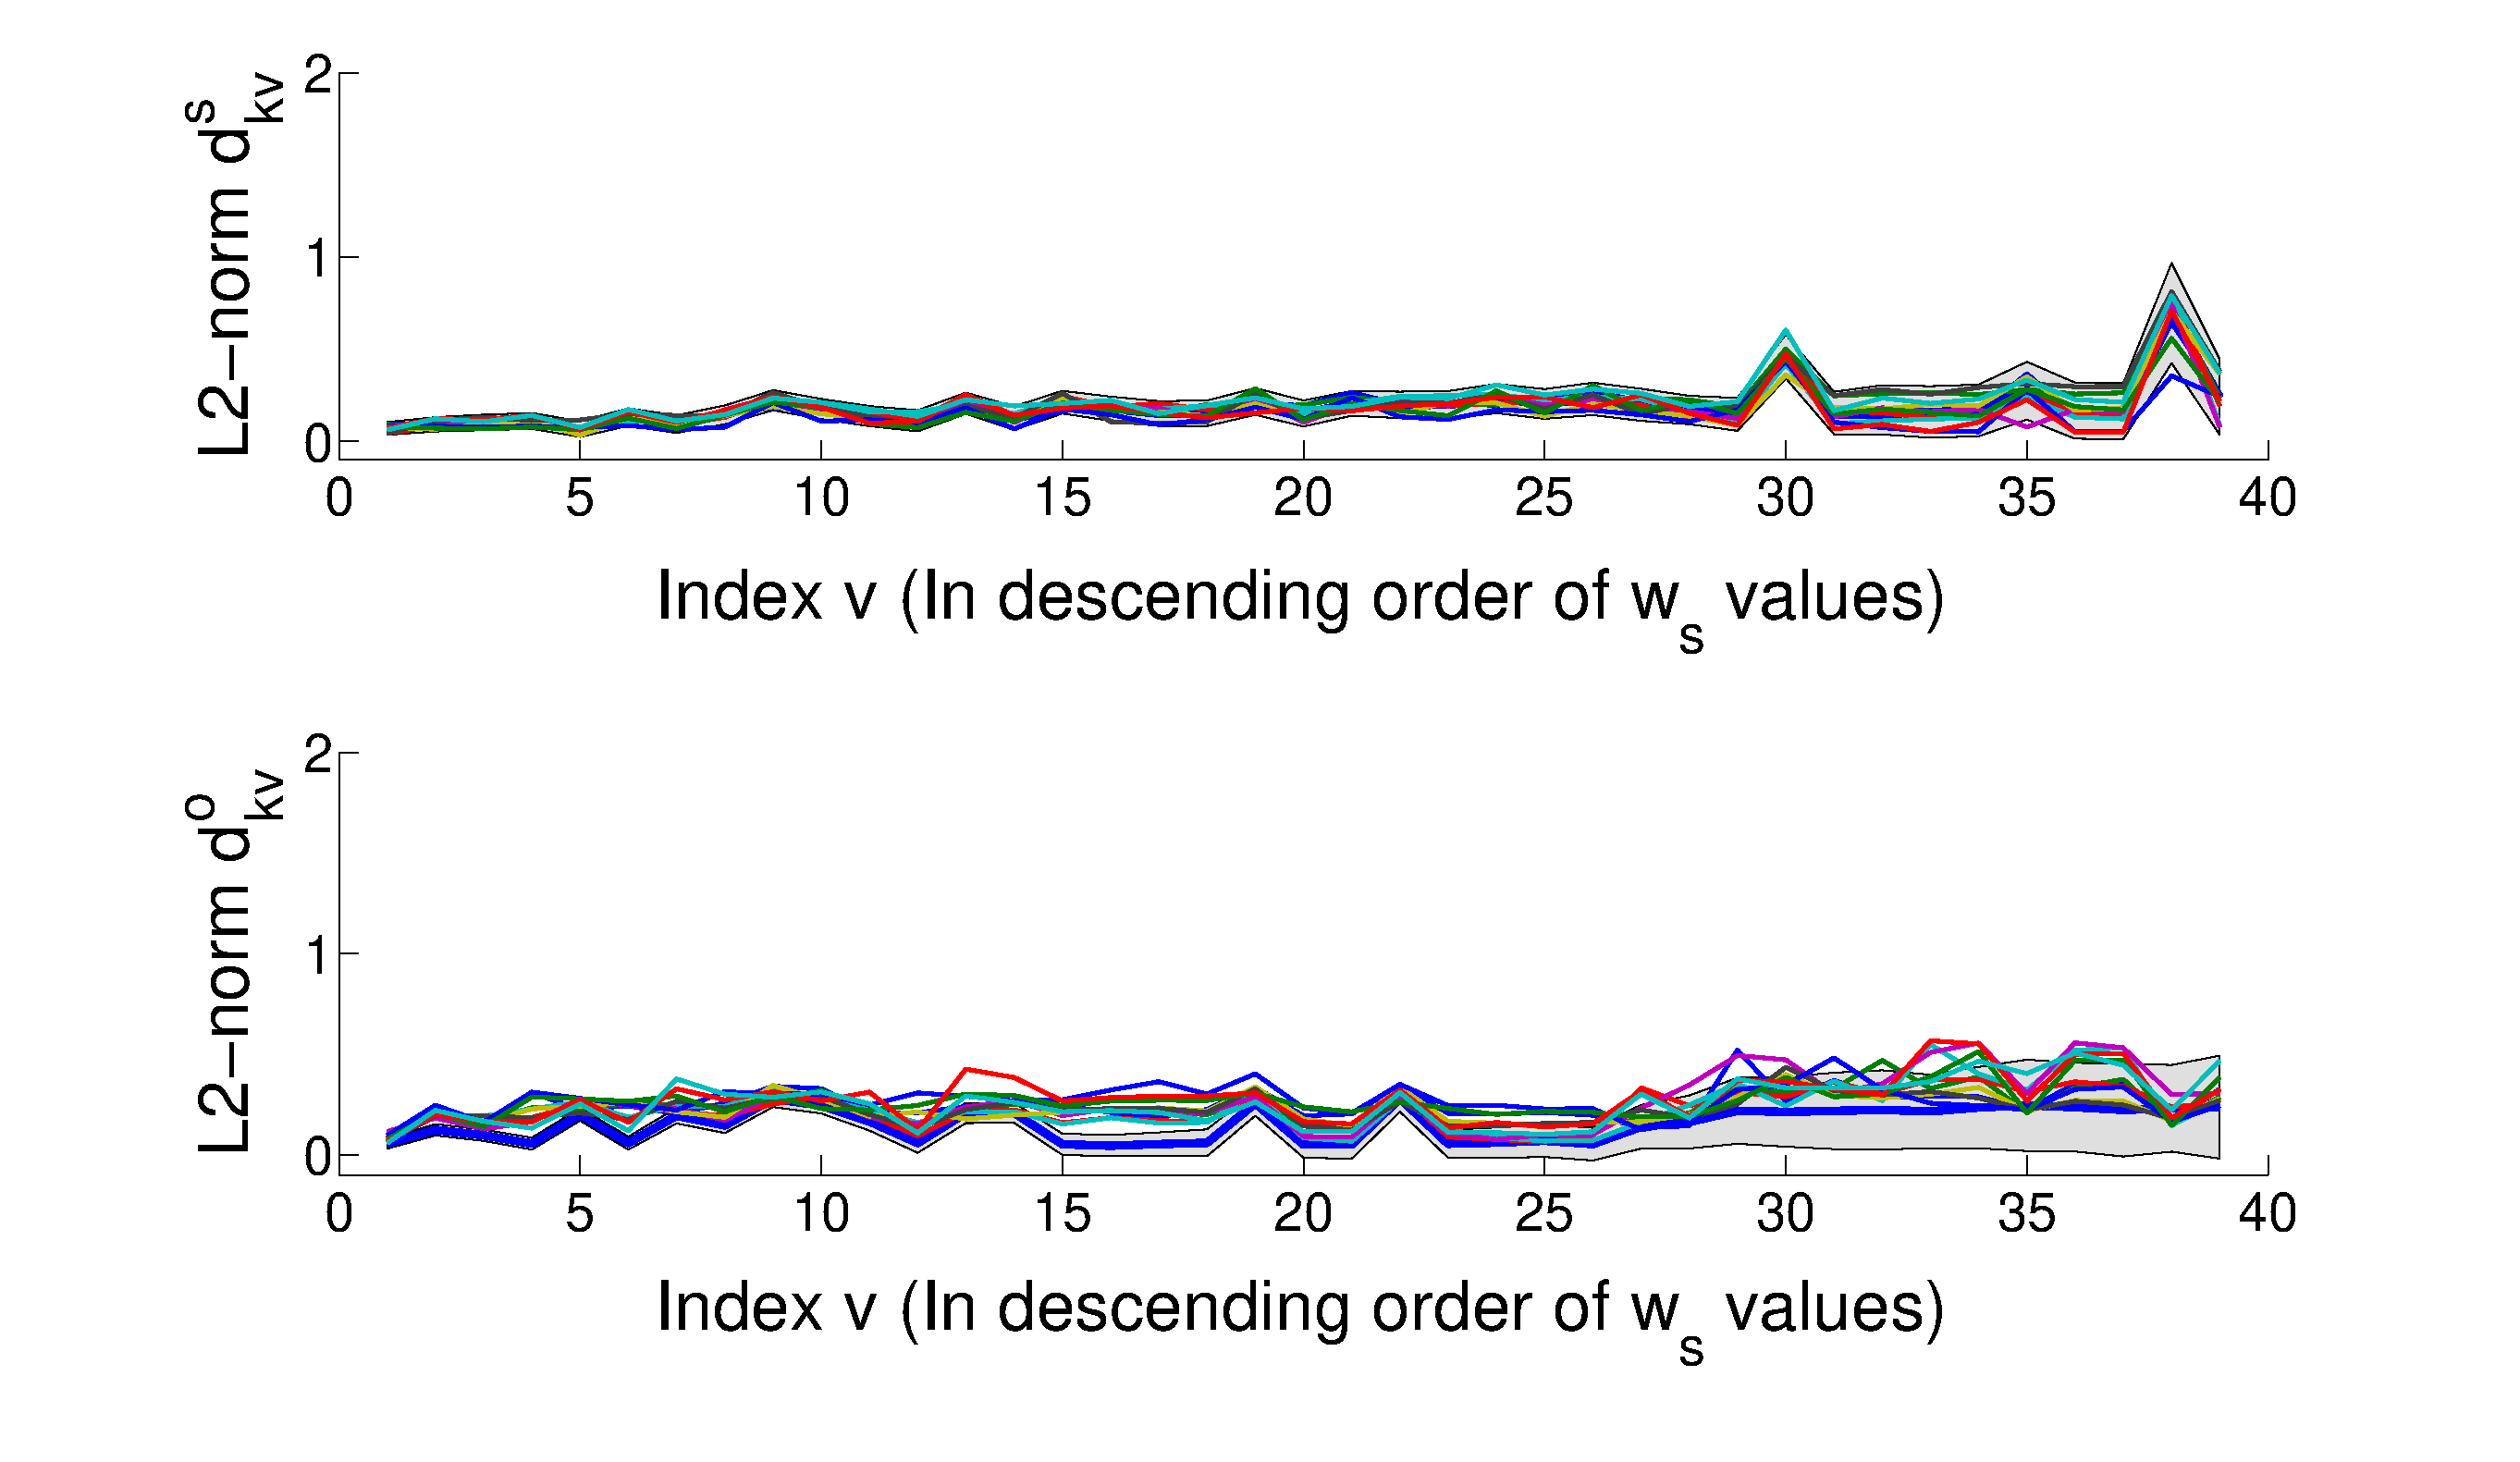
\includegraphics[width=\textwidth, trim={0.5cm 0 3.8cm 0}, clip]{strawberry_learning_results}
      \caption{}
      \label{fig:feat_results_strawberry}
  \end{subfigure}
  \vskip -2pt
  \begin{subfigure}[]{0.6\textwidth}
      \hskip -0.5cm
      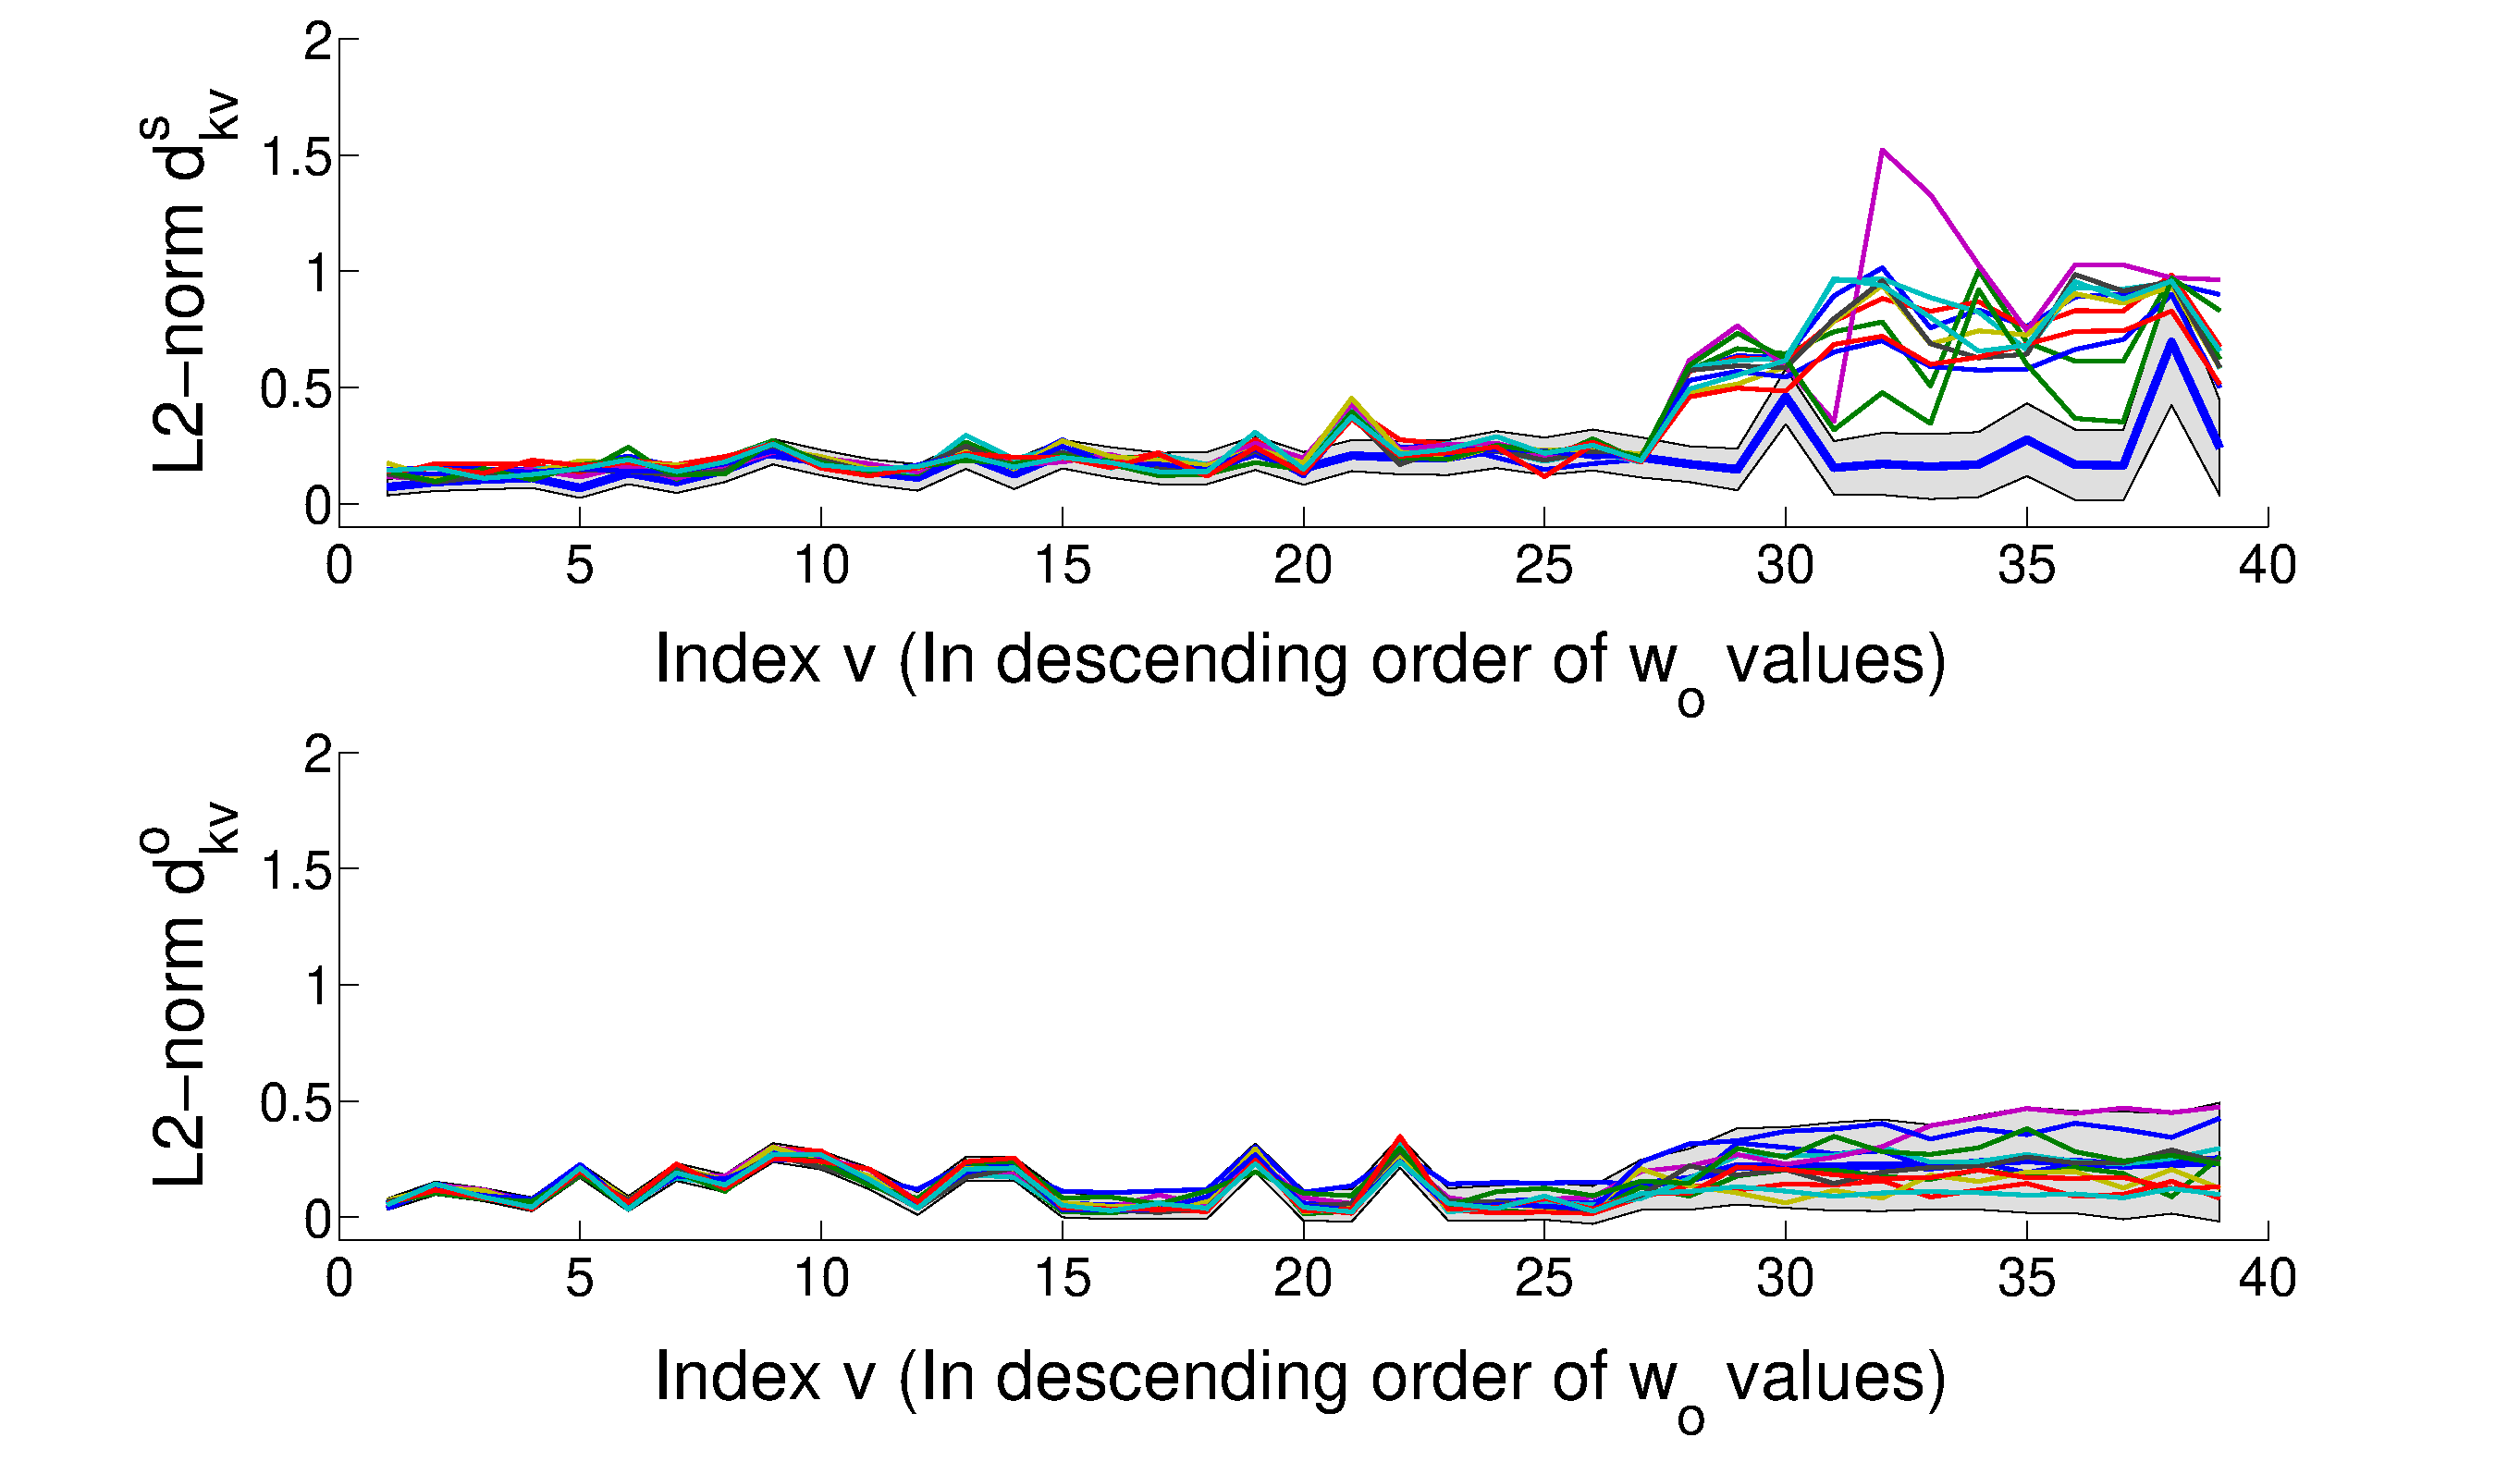
\includegraphics[width=\textwidth, trim={0.5cm 0 3.8cm 0}, clip]{orange_learning_results}
      \caption{}
      \label{fig:feat_results_orange}
  \end{subfigure}
\caption[Validation results showing the conformance of the specimens to the learnt feature distributions]{Results obtained by using the learning dataset for testing. The plots in \subref{fig:feat_results_strawberry} shows the 13 starwberry specimens evaluated against the feature distribution sequences of Strawberry $F_s$ (top plot of \subref{fig:feat_results_strawberry} or \subref{fig:feat_results_strawberry}-top) and Orange (bottom plot of \subref{fig:feat_results_strawberry} or \subref{fig:feat_results_strawberry}-bottom). The feature distribution represented here with mean shown as a solid blue line with the 95\% confidence interval shown as a grey band around the mean is an alternate representation of Figure~\ref{fig:feat_distr_strawberry}. The sequence of feature distributions indexed by $v$ here is arranged in the decreasing order of importance as dictated by the Strawberry feature weights $W_s$. Since the results shown in \subref{fig:feat_results_strawberry} are only for Strawberry specimens both the 
Strawberry distribution (\subref{fig:feat_results_strawberry}-top) and Orange distribution (\subref{fig:feat_results_strawberry}-bottom) are ordered using the Strawberry feature weights $W_s$. The colored lines in \subref{fig:feat_results_strawberry} are the $D^s_k$ values (in \subref{fig:feat_results_strawberry}-top) and $D^o_k$ (in \subref{fig:feat_results_strawberry}-bottom) for the different Strawberry specimens. 
The plots in \subref{fig:feat_results_orange} are similar to \subref{fig:feat_results_strawberry}, except that they are the evaluation results of Orange specimens against Strawberry feature sequence $F_s$ (\subref{fig:feat_results_orange}-top) and Orange distribution sequence $F_o$ (\subref{fig:feat_results_orange}-bottom). The indices $v$ in \subref{fig:feat_results_orange} are arranged in the decreasing order of Orange feature weights $W_o$. Both Orange and Strawberry specimens matching with most distributions of their corresponding class is a visual indicator validating the machine learning solution developed in this chapter.}
\label{fig:feat_results}
\end{figure*}	
%

A more concrete validation of the machine learning approach discussed in this paper is by computing the \emph{class confidence} $H^s_k$ and $H^o_k$ of each specimen against the Strawberry and Orange classes respectively and deciding on the class of the specimen as described in Section~\ref{sec:distdes_validation}. One thing to note here is that the class confidence measure is a comparison of a specimen against the Strawberry and Orange feature distribution sequences one of which utilized the specimen images while it was evaluated. It is a general rule to separate the learning and testing datasets before validating a machine learning approach. In this case, since the data set consists of only 24 specimens, a leave-one-out cross-validation\footnote{Leave-one-out cross-validation is used in cases where the number of specimens available is very small which makes if ineffective to split the available labeled dataset into learning and testing sets. In leave-one-out cross-validation, during each iteration 1 
specimen is chosen as the testing set and the all other specimens are chosen as the learning set resulting in repeatedly performing the learning procedure for each iteration.} \cite{alpaydin} was implemented. The class confidence values $H^s_k$ and $H^o_k$ of the 13 Strawberry specimens are shown as black and red bars respectively in Figure~\ref{fig:results_strawberry}. Its clear that the black bars are taller than the red bars in all cases. According to hypothesis test \eqref{eqn:hypothesis_test}, this impies that that all Strawberry specimens are classified correctly. The same can be said for the results from Orange specimens in Figure~\ref{fig:results_orange}, since all the red bars are taller than the back bars, all the orange specimens are also classified correctly.

%
\begin{figure*}
  \centering
  \begin{subfigure}[]{0.7\textwidth}
      \includegraphics[width=\textwidth]{classification_metric_strawberry}
      \caption{}
      \label{fig:results_strawberry}
  \end{subfigure}
  \vskip -2pt
  \begin{subfigure}[]{0.7\textwidth}
      \includegraphics[width=\textwidth]{classification_metric_orange}
      \caption{}
      \label{fig:results_orange}
  \end{subfigure}
\caption[Classification results]{}
\label{fig:results}
\end{figure*}	
%

The validation procedure confirms the ability of this machine learning technique to combine data from multiple images of a specimen to do a binary classification task. The 24 specimens collectively belonging to Starwberry and Orange classes were correctly classified by the machine learning algorithm developed here.

%================================================================================================================
\section{Discussion}
\begin{enumerate}
	\item The plots of the feature descriptor clearly show their conformance only to the feature distribution of the target class they belong to.
	
	\item Though capturing multiple images of a target object from different height could slowdown the imaging process and impose additional constrains on the object recognition process, detecting critical targets from noisy images justifies this end.
\end{enumerate}

The machine learning approach developed here was used to perform binary classifcation on a set of 22 specimens containing an assortment of Strawberry and Orange specimens. The graphical results from Figure~\ref{fig:feat_results} clearly show the conformance of the distance measures $D^s_k$ and $D^o_k$ of specimens only to the respective class they belong to. This is further reinforced by the class confidence measures $H^s_k$ and $H^o_k$ clearly assigning each specimen to their right class. Ultimately, all the specimens were classified correctly hence achieving a 100\% precision and recall rates.\footnote{\label{1} \emph{Precision} and \emph{Recall} are performance measures for a machine learning algorithm. Precision is the ratio of true positives to the total number of detections and recall is the ratio of true positives to the total number of positives in the dataset.} 

The theoretically best possible performance obtained here portrays the potential of this algorithm to work in noisy natural images. One source of noise in the data collection process was floating specks of dust in the water also dust on the floor of the tank. There were even instances when the foot of the person operating the imaging-rig was included in the images collected. The uncontrolled lighting introduced light artifacts and uneven illumination in the image which also acted as an additional source of noise. The effect of uneven lighting conditions faced during data collection process is clearly visible in Figure~\ref{fig:height_specimen}. The ability of this algorithm to generate outstanding results even in the presence of noise offers great confidence on its ability to handle unpredictable environmental conditions.

Since only 22 objects were used for evaluation, it will be an intersting study to test this algorithm on a natural image dataset containing a few thousand specimens. The requirement of multiple images of the same specimen from different heights and the associated annotation on a large learning set might appear cumbersome. However the semi-automated annotation procedure provided in Section~\ref{sec:distdes_annotation} alleviates the manual labor involved to a small fraction of what will be required for a full fledged annotation effort on an entire dataset containing multiple images for each specimen.

Since this approach relies on multiple images for each specimen, imaging time and effort involved is higher than an object recognition algorithm that is designed to operate on a single image of a specimen. The use of multiple images and 39 hypothesis tests (see Section~\ref{sec:distdes_validation}) help to decide on the identity of a target specimen with higher confidence than an approach that just uses a single image of a target. Multiple images offer a way to extract features from different scales of an object which when combined together offer a robust object recognition framework. In cases where it is critical to classify a target with confidence, for instance in case of detecting unexploded mines or submerged ordinance, such an approach that is accurate is  valuable despite the additional imaging time incurred.

%================================================================================================================
\section{Conclusion}
\begin{enumerate}
        \item The developed technique offers a way to detect objects from noisy images without any segmentation using images of a target captures from different height.
\end{enumerate}

The machine learning method developed here offers a way to perform binary classification using global descriptors generated from multiple images of a specimen. This technique was successful in recognizing all the 22 specimens available in our dataset of 11 Strawberries and 11 Oranges. The performance of this technique on this dataset is the absolute theoretical maximum that can be obtained for a machine learning technique. This exceptional performance despite the presense of noise and several uncontrolled variables in the data collection process is indicative of the robustness of this algorithm. Additionally, the ability of this algorithm to perform object recognition via histogram based global descriptors, avoids segmentation entirely. Since segmentation can be problematic in noisy images where the edges of objects is hard to determine, doing away with segmentation is a great incentive to adopt this technique for noisy images.
%================================================================================================================
\section{Future work}

This algorithm has been tested on a set of 22 images collected using an imaging rig. It will be interesting to exand this technique to natural datasets where multiple instances of the same target object have been captured. The current procedure adopted here computes a set of discrete measurements from a fixed set of heights from which images are available. Expanding this to work with an arbitrary but known set of heights will be valuable for object recognition tasks where the data collected cannot adhere to such predetermined heights. Expaning this binary classification problem into a multiclass classification for a larger number of object classes is another natural direction that can be explored.

%================================================================================================================

\printglossary[type=\acronymtype]                  
%
% This is the Bibliography file (bibtex.tex)
% This generally works for BibTeX

% Use sample.bib for BibTeX database
\bibliography{thesis_ref}
% BibTeX style (plain, alpha, unsrt)
\bibliographystyle{plain}
   % This file (bibtex.tex) contains the text
                   % for a bibliography if using BibTeX with
                   % sample.bib
\end{document}


